\chapter{Application to Markov chain Monte Carlo algorithms}
\label{ch:mcmc}
One of the interesting applications of $\gradTD$ learning is in the context of Markov chain Monte Carlo(MCMC) simulations. In this chapter, a basic introduction to MCMC algorithms with a particular emphasis on Langevin diffusion and its discrete variants is provided first in \Section{s:mcmc_langevin}. We then define asymptotic variance as a measure of convergence and motivate how $\gradTD$ learning is perfectly suited to obtain MCMC estimates with minimal asymptotic variance. In \Section{s:mcmc_metropolis}, we introduce the very popular Metropolis-Hastings (MH) algorithm and present an extension of the asymptotic variance reduction methods to the class of reversible Markov chains in \Section{s:mcmc_reversible_mc_cv}. A majority of the existing research that aims to improve the convergence of MCMC estimates focus on minimizing the sample variance, as it is easier to implement. In \Section{s:mcmc_var_vs_asym_var}, through a motivating example, we prove why this is not the correct objective for MCMC. 
In recent research, it has been found that under certain assumptions, the convergence rates of ULA and RWM are related and the same asymptotic variance reduction techniques can be applied to RWM \cite{brodurmeymourad18}. \anand{Need to rephrase after reading \cite{brodurmeymourad18}} Applications to numerical examples involving logistic regression (logit) and probit models are discussed in \Section{s:mcmc_numerics}. 

\section{Langevin Diffusion for MCMC}
\label{s:mcmc_langevin}
In many scenarios, it is of interest to compute the expectation of a function $c$ with respect to a target distribution $\pr$:
\begin{equation}
\eta = \int c(x)\pr(x)\ud x\, .
\label{e:eta}
\end{equation} 
Typically, computing integrals of the form \eqref{e:eta} analytically is difficult when $\pr$ is in high dimensions and Markov chain Monte Carlo (MCMC) methods are used instead. MCMC provides numerical algorithms to obtain estimates of $\eta$. It can be approximated using time averages of the following form:
\begin{equation}
\eta_N =\frac{1}{N}\sum_{n=0}^{N-1} c(\markovstate_n),
\label{e:sample_mean_HM}
\end{equation}
in which $\boldsymbol{\markovstate}$ is a Markov chain whose steady-state distribution has density $\pr$ \cite{asmgly07,MT}.
In this chapter, we initially focus on a formulation in continuous time and then extend the idea to discrete-time MCMC algorithms.

The Langevin Diffusion, introduced in \Section{s:langevin_diffusion} is the grandmother of all MCMC algorithms. It forms the basis for various other popular MCMC algorithms such as the unadjusted Langevin algorithm (ULA) and Metropolis-adjusted Langevin algorithm (MALA). The diffusion obeys the stochastic differential equation in \eqref{e:diff_td_langevin_cts}:
\begin{equation}
\ud \markovstate_t = - \nabla \pot(\markovstate_t) \, \ud t+  \sqrt{2} \, \ud W_t,
\label{e:mcmc_langevin_cts}
\end{equation}
where $\bfmW=\{W_t : t\ge 0\}$ is a standard Brownian motion on $\Re^d$.
Under general conditions, this diffusion is reversible, with unique invariant density $\pr=e^{-U +\Lambda}$,  where $\Lambda$ is a normalizing constant so that $\pr$ integrates to unity.  For a large $T$, the mean $\eta$ can be approximated as,
\begin{equation}
\eta \approx \eta_T \eqdef \frac{1}{T}\int_0^T c(\markovstate_t) \, dt.
\label{e:mcmc_lang_mean_cts}
\end{equation}

To compare the different MCMC algorithms it  is convenient to consider an asymptotic setting.   Under general conditions, the estimates will obey a Central Limit Theorem (CLT) of the form:
\begin{equation}
\sqrt{T} \tileta_T \xrightarrow[]{d} N(0,\asymvar^2)
\end{equation}
where $\tileta_T =\eta_T-\eta$, and the convergence is in distribution.   Under further mild assumptions,  the variance of the Gaussian limit is given by the so-called asymptotic variance:
\begin{equation}
\asymvar^2 = \lim_{T \to \infty} \Expect \left[\left(\frac{1}{\sqrt{T}}\int_{0}^{T}(c(\markovstate_t)-\eta)dt\right)^2\right]
\label{e:aVar}
\end{equation}
For example, these conclusions hold for a Markov chain that is $V$-uniformly ergodic,  provided $c^2\in\LV$  \cite{glymey96a,MT}. \anand{$c^2$ or $c$?}
It has been shown in \cite{glymey96a,MT} that the asymptotic variance $\asymvar^2$ has the following general representation in terms of the solution to Poisson's equation $h$ \eqref{e:diff_td_poissons},
\begin{equation}
\asymvar^2  =2\langle h, \tilc\rangle_{L^2}.
\label{e:avarFish}
\end{equation}
The representation \eqref{e:avarFish} is valid for any diffusion that is $V$-uniformly ergodic.
For the special case of the Langevin diffusion,  by application of \Prop{prop:lang_generator_grad}, $\asymvar^2 = 2 \| \nabla h \|^2_{L^2}$.

The primary goal in the design of MCMC algorithms is the faster convergence of the Markov chain to its invariant distribution (i.e. the target distribution). The asymptotic variance is a measure of this convergence and hence, it is ideal to minimize $\asymvar^2$. Several approaches have been proposed to improve the convergence rate including constructing an irreversible Markov chain with the same invariant density \cite{hwanorwu15, dunlelpav16}, using an optimal scaling parameter \cite{robros01} etc. Most of these approaches alter the transition kernel of the Markov chain and hence, do not work well on samples already obtained. In the remainder of this paper, we restrict our discussion to post-hoc schemes for reversible Markov chains, i.e. samples from an ergodic Markov chain are available and variance reduction is achieved by post-processing. These scheme require no changes to the sampling methodology. 

Control variates introduced in \cite{HenThesis,henmeytad03a,kimhen07,ctcn} are zero-mean terms, which when added to the estimator can produce a significant reduction in the asymptotic variance without adding bias. One of the advantages of this scheme is that they work post-hoc, and are independent of the MCMC algorithm used. \anand{a few more words on original application}

Dellaportas et al. in \cite{delkon12} have employed control variates for particular examples of reversible Markov chains like the Gibbs sampler.
More recently, Brosse et al. in \cite{brodurmeymou18} show that the asymptotic variances of ULA, MALA and RWM are close to the asymptotic variance of the Langevin diffusion and construct control variates that work for all the three methods. In this dissertation, we borrow heavily from both the above and demonstrate that using RKHS based $\gradTD$ learning algorithms, the variance reduction is improved many-fold. 

The basic idea is described here. Let $\psi\colon\Re^d\to\Re^\ell$ denote a $C^2$ function, regarded as a family of $\ell$ basis functions, and $\param\in\Re^\ell$ denote the parameters,
\begin{equation}
\begin{aligned}
c^\param  \eqdef c + \underbrace{\generate h^\param}_{\text{Control variate}},
\qquad
\text{where}
\quad
h^\param  \eqdef  \sum_{i=1}^\ell \param_i \psi_i = \param^\transpose \psi\,
\end{aligned}
\label{e:mcmc_h_and_c}
\end{equation}
and $\generate$ denotes the differential generator of the Langevin diffusion \eqref{e:diff_td_langevin_generator}. 
Under the assumptions imposed it will follow that the steady-state means of $c$ and $c^\param$ coincide for any $\param\in\Re^\ell$,  so that we obtain a family of asymptotically unbiased estimators: \anand{Do we need to show $Ph = h$?}
\begin{equation}
\eta^\param_T =\frac{1}{T}\int_0^T c^\param(\markovstate_t)  \, dt
\label{e:mcmc_eta_theta}
\end{equation}
It is then of interest to find the parameter with minimal asymptotic variance:
\begin{equation}
\param^* = \argmin_\param (\asymvar^\param)^2
\label{e:mcmc_theta_star}
\end{equation}
Here, $(\asymvar^\param)^2$ corresponds to the asymptotic variance of the new estimate \eqref{e:mcmc_eta_theta}, i.e.
\[
\sqrt{T} (\eta^\param_T - \eta ) \xrightarrow[]{d} N (0,(\asymvar^\param)^2).
\]

\begin{proposition}
	\label{t:mcmc_say_var_cv}
	Suppose that  $c$ and each $\psi_i$ lie in $\LsqrV$. Then, equation \eqref{e:mcmc_eta_theta} defines an asymptotically unbiased estimate of $\eta$. Its asymptotic variance is
	\begin{equation}
	(\asymvar^\param)^2
	= 2  \| \nabla  h - \nabla h^\param  \|^2_{L^2}
	\label{e:mcmc_asy_var_cv}
	\end{equation}
\end{proposition}

\begin{proof}
	Applying the differential generator $\generate$ on $h - h^\param$, we have
	\begin{equation}
	\begin{aligned}
	\generate ( h -h^\param) & = - \tilc - \generate h^\param\\
	& = - c + \eta + c - c^\param  \qquad \text{From \eqref{e:mcmc_h_and_c}} \\
	& = - c^\param + \eta\, \eqdef -\tilc^\param
	\end{aligned}	
	\label{e:mcmc_proof_i}
	\end{equation}
	Hence $h-h^\param$ is the solution to Poisson's equation with forcing function $c^\param$. Analogous to \eqref{e:avarFish}, the asymptotic variance for the new estimator in \eqref{e:mcmc_eta_theta} is represented as $(\asymvar^\param)^2 = 2 \langle h - h^\param, \tilc^\param \rangle_{L^2}$, and applying \Prop{prop:lang_generator_grad} gives \eqref{e:mcmc_asy_var_cv}.
\end{proof}

An important observtion here is that the asymptotic variance $(\asymvar^\param)^2$ for the new estimator \eqref{e:mcmc_h_and_c}, with control variates \eqref{e:mcmc_asy_var_cv} has the same form as \eqref{e:diff_td_gradTD_norm_error}, and hence any of the variants of the $\gradTD$ algorithm can be applied. Numerical examples using these algorithms are discussed in \Section{s:mcmc_numerics}.

\section{Metropolis-Hastings algorithm}
\label{s:mcmc_metropolis}
Although Langevin diffusion offers a very intuitive sampling algorithm, it requires the computation of the gradient of the potential function $U$, which may be expensive in high dimensions. Hence, other discrete time algorithms are preferred. Metropolis-Hastings algorithm is a popular MCMC technique to simulate multivariate distributions. It was originally proposed by Metropolis in 1953 and extended to a more general case by Hastings in 1970 \cite{has70}. The only requirement in Metropolis-Hastings is that it should be possible to compute the value of a function $f$ proportional to the target density $\pr$. The function $f$ could potentially be the unnormalized form of $\pr$.

The algorithm requires the choice of a simple ``proposal'' distribution $g$, from which samples can be drawn easily. The function $g(x,y)$ gives the conditional distribution for the next sample $y$, given the current sample $x$.  The algorithm can be summarized in the following steps:

\begin{itemize}
	\item Choose an arbitrary point $\markovstate_0 = x$ to be the first sample.
	\item Choose a proposal distribution $g$. Pick a new candidate sample point $x' \sim g (x,.) $.
	\item Compute the acceptance ratio $\alpha(x,x')= \min \left[ \frac{f(x') \, g (x',x)}{f(x) \, g(x,x')}, 1\right] $.
	\item With probability $\alpha$, accept $x'$ and set $\markovstate_1 = x'$; if rejected set $\markovstate_1 = x$.
	\item Repeat above for $ \markovstate_2, \hdots \markovstate_N$ for a fixed $N$.
\end{itemize}
% If $g$ is chosen to be Gaussian, due to symmetry $g(x,y) = g(y,x)$. This simplifies the computation of the acceptance ratio $\alpha$.

The transition kernel $P_{mh}$ for a Metropolis-Hastings chain can be written as:
\begin{equation}
P_{mh}(x,dy) \eqdef g(x,y) \alpha(x,y) dy + \left [ 1 - \int_{\state} g(x,y) \alpha(x,y) dy \right] \delta_x (dy),
\label{e:kernel_mh}
\end{equation}
and with the acceptance ratio $\alpha$ as defined, the reversible Markov chain with kernel $P_{mh}$ has its invariant density as $\rho$.

A special case of this algorithm is obtained if $g$ is chosen to be a Gaussian centered at $x$ with $\gamma$ as the variance parameter. This also simplifies the expression for $\alpha$ as $g(x,x') = g(x',x)$. This variant is known as the random walk Metropolis (RWM) algorithm. For a small value of $\gamma$, it has been shown by Brosse et al. in \cite{brodurmeymourad18} that the following relation between $P_{mh}$ and the differential generator $\generate$ of the Langevin diffusion holds,
\[
\lim_{\gamma \to 0} \gamma^{-1} (P_{mh} - I) = \generate
\]
Thus for small values of $\gamma$, the control variates can be obtained as $\gamma \generate h^\theta$. \rd{But this approximation is not valid for larger step-sizes and hence this method is practically limited in use.} \notes{Do we need this statement? Or is there a hack for larger $\gamma$? }

\section{Control Variates for a Reversible Markov Chain} 
\label{s:mcmc_reversible_mc_cv}
In this section, we extend the idea of control variates to the more general case of reversible Markov chains, including RWM. The main difficulty is that \Prop{prop:lang_generator_grad} is absent here. However using reversibility, we obtain an expression for the optimal parameter values. A derivation similar to this is presented in \cite{delkon12}.
Consider a discrete time Markov chain with a transition kernel $P$.  Let $h$ denote the solution to the Poisson's equation of this Markov chain,
\[
(P - I) h = -\tilc,
\]
where $I$ refers to the identity operator.
In discrete time, the asymptotic variance has the following representation in terms of $h$,
\begin{equation}
\asymvar^2 = 2 \langle h, \tilc \rangle_{L^2} - \langle \tilc, \tilc \rangle_{L^2}.
\label{e:mcmc_avar_reversible}
\end{equation}
A linearly parameterized class of functions $h^\param$ is defined as in \eqref{e:mcmc_h_and_c} and a new function $c^\param$ with the control variates is defined as
\begin{equation}
c^\param \eqdef c +  (P - I) h^\param
\label{e:mcmc_discrete_cv}
\end{equation}
Denoting $\tilh^\param \eqdef h - h^\param$, a simple extension of \eqref{e:mcmc_proof_i} is obtained:
\begin{equation}
(P - I) \tilh^\param = -\tilc^\param.
\label{e:mcmc_discrete_poissons_cv}
\end{equation}
Following from \eqref{e:mcmc_avar_reversible}, the asymptotic variance corresponding to this new estimator $c^\param$ has the following representation:
\begin{equation}
\begin{aligned}
(\asymvar^\param)^2 \eqdef & 2 \langle \tilh^\param, \tilc^\param \rangle_{L^2} - \langle \tilc^\param, \tilc^\param \rangle_{L^2}\\
= &  - 2 \langle \tilh^\param, (P - I) \tilh^\param \rangle_{L^2} -\langle (P - I) \tilh^\param, (P - I) \tilh^\param \rangle_{L^2}\\
= & \langle \tilh^\param, \tilh^\param \rangle_{L^2} - \langle P \tilh^\param, P \tilh^\param \rangle_{L^2}
\label{e:mcmc_asym_var_theta_discrete}
\end{aligned}
\end{equation}
To eliminate the unknown term $h$ from \eqref{e:mcmc_asym_var_theta_discrete}, the self-adjoint property of the transition kernel of a reversible Markov chain is used (\Prop{theorem:self_adjoint}).
\begin{proposition}
	\label{theorem:self_adjoint}
	For a reversible Markov chain the following holds:
	\[
	\langle P f , g \rangle_{L^2}= \langle f, P g \rangle_{L^2}, \qquad f,g \in L^2(\pr)
	\]
\end{proposition}
\begin{proof}
	For a reversible Markov chain, the detailed balance equations hold with respect to its unique invariant measure $\pr$:
	\begin{equation}
	\pr(dx) P(x,dy ) = \pr(dy) P(y,dx).
	\label{e:det_bal}
	\end{equation}
	From the definition of the transition kernel $P$,
	\begin{equation}
	\begin{aligned}
	P f (x) & = \Expect [f(\markovstate_{k+1}) | \markovstate_k = x] \\
	& = \int P(x,dy) f(y)
	\label{e:trans_kernel}
	\end{aligned}
	\end{equation}
	Using the definition of the inner product,
	\[
	\begin{aligned}
	\langle P f, g \rangle_{L^2} & \eqdef \int (Pf(x)) g(x) \pr(dx) \\
	& = \int \left(\int P(x,dy)f(y)\right) g(x) \pr(dx)  \qquad (\text{From } \eqref{e:trans_kernel}) \\
	& = \int \left(\int P(y,dx) g(x) \right) f(y) \pr(dy) \qquad (\text {Applying } \eqref{e:det_bal})\\
	& = \int (P g(y)) f(y) \pr(dy) \\
	& = \langle f, P g \rangle_{L^2}.
	\end{aligned}
	\]
\end{proof}

\begin{proposition}
	\label{t:theta_discrete}
	The optimal parameter vector $\param^* \in \Re^\ell$ that minimizes \eqref{e:gamma_discrete} is given by
	\begin{equation}
	\begin{aligned}
	\param^* & \eqdef M^{-1} b \qquad \text{where,} \\
	M &\eqdef \langle \psi, \psi \rangle_{L^2}- \langle P \psi,  P \psi \rangle_{L^2} \\
	b & \eqdef  \langle \tilc, \psi \rangle_{L^2} +  \langle \tilc, P \psi \rangle_{L^2}.
	\end{aligned}
	\label{e:theta_star_discrete}
	\end{equation}
	The optimal control variate is then given by,
	\[
	(P-I) h^\param = \param^{* \transpose} (P \psi) - \param^{* \transpose} \psi.
	\]
\end{proposition}
\begin{proof}
	Expanding the expression for $(\asymvar^\param)^2$ \eqref{e:mcmc_asym_var_theta_discrete} gives,
	\begin{equation}
	\begin{aligned}
	(\asymvar^\param)^2 & = \langle \tilh^\param, \tilh^\param \rangle_{L^2} - \langle P \tilh^\param, P \tilh^\param \rangle_{L^2} \\
	& = \langle h, h \rangle_{L^2} - 2 \langle h, h^\param \rangle_{L^2} + \langle h^\param , h^\param \rangle_{L^2} - \langle P h, P h \rangle_{L^2} + 2 \langle P h , P h^\param \rangle_{L^2} - \langle P h ^\param , P h^\param \rangle_{L^2}
	\label{e:gamma_discrete}
	\end{aligned}
	\end{equation}
	Substituting for $h^\param$ in \eqref{e:mcmc_asym_var_theta_discrete} and applying the first order necessary conditions for optimality by taking the derivative with respect to $\param$,
	\begin{equation}
	\begin{aligned}
	0 & = - \langle h, \psi \rangle_{L^2} +  \param^{*\transpose} \langle \psi, \psi \rangle_{L^2}+ \langle P h, P \psi \rangle_{L^2}-\param^{*\transpose}  \langle P \psi, P  \psi \rangle_{L^2}  \\
	& = - \langle h, \psi \rangle_{L^2} +  \param^{*\transpose} \langle \psi, \psi \rangle_{L^2}+ \langle P h, P \psi \rangle_{L^2}-\param^{*\transpose}  \langle P \psi, P  \psi \rangle_{L^2}  + \langle P h, \psi \rangle_{L^2} - \langle P h, \psi \rangle_{L^2} \\
	& = - \langle \tilc , \psi \rangle_{L^2} + \langle P h, (P - I) \psi \rangle_{L^2} + \param^{*\transpose} \Bigl( \langle \psi, \psi \rangle_{L^2}  - \langle P \psi, P \psi \rangle_{L^2} \Bigr) \qquad \text{(Using $(P-I) h = -\tilc$)}
	\label{e:mcmc_gradient_reversible}
	\end{aligned}
	\end{equation}
	Applying \Prop{theorem:self_adjoint},
	\[
	\langle P h , (P -I) \psi \rangle_{L^2} = \langle (P - I) h, P \psi\rangle_{L^2} = - \langle \tilc, P \psi \rangle_{L^2}
	\]
	Denoting $M$ and $b$ as
	\[
	M \eqdef \langle \psi, \psi \rangle_{L^2} - \langle P \psi, P \psi \rangle_{L^2}, \qquad b \eqdef \langle \tilc, \psi \rangle_{L^2} + \langle \tilc, P \psi \rangle_{L^2}.
	\]
	completes the proof.
\end{proof}
It can be shown that $M$ is a symmetric positive definite matrix. The Monte Carlo estimates of $M$ are designed to respect this constraint:
\[
\begin{aligned}
\hat{M}_N & \eqdef \frac{1}{N} \sum_{n=0}^{N-1} \Bigl(\psi(\markovstate_n) \cdot\psi^\transpose(\markovstate_n) - \psi(\markovstate_{n+1})\cdot \psi^\transpose(\markovstate_{n+1}) \Bigr) \\
M_N  & \eqdef \frac{1}{2} (\hat{M}_N + \hat{M}_N^\transpose )\\
b_N & \eqdef  \frac{1}{N} \sum_{n=0}^{N-1} \tilc(\markovstate_n)\, \Bigl( \psi(\markovstate_n) + \psi(\markovstate_{n+1}) \Bigr).
\end{aligned}
\]

Similar results for optimal control variates for reversible Markov chains have been obtained in \cite{delkon12}. Although optimal parameter weight estimates $\param_N = M_N^{-1} b_N$ are easy to obtain, the main difficulty is to compute the term $P\psi$ which is part of the control variate defined in \Prop{t:theta_discrete}. In \cite{delkon12}, numerical examples are presented for a class of conjugate random-scan Gibbs samplers for which $P\psi$ is explicitly computable in closed form. In this dissertation, we substitute for $(P-I)\basis$ with $\gamma \generate \basis$, which is easy to compute. Recent results in \cite{brodurmeymourad18} justifies this substitution for small values of $\gamma$. 

\section{Sample Variance v Asymptotic Variance}
\label{s:mcmc_var_vs_asym_var}
The basic idea behind using control variates to minimize asymptotic variance of the MCMC estimates was discussed in \Section{s:mcmc_langevin}. It requires approximating the value function $h$, which is non-trivial in most cases. A large body of prior research \cite{oatgircho,papmirgir14} attempts to achieve better estimates by solving an easier problem. In \cite{papmirgir14}, a parameterized family of control variates is considered as in this dissertation. However, the optimal parameter is chosen to minimize the sample variance rather than the asymptotic variance. This is well-motivated only  if the samples are i.i.d. 
The unbiased estimator in \cite{papmirgir14} is based on a function $c^{\vartheta}$ of the same form as \eqref{e:mcmc_h_and_c}:
\[
\begin{aligned}
c^\vartheta  \eqdef c + \generate h^\vartheta,
\qquad
\text{where}
\quad
h^\vartheta  =  \sum_{i=1}^\ell \vartheta_i \psi_i = \vartheta^\transpose \psi.\,
\end{aligned}
\]
%Examples include the paper by Oates et al. \cite{oatgircho}, where the problem considered is the minimization of sample variance by using a new estimator  chosen from within Reproducible kernel Hilbert space (RKHS), and the paper by Mira et al \cite{papmirgir14}, which is similar to the present work.
The quantity minimized is the sample variance, i.e. $(\sigma^\vartheta)^2 = \Expect[(\tilc^{\vartheta})^2] = \langle \tilc^\vartheta, \tilc^\vartheta \rangle_{L^2}$, where $\tilc^\vartheta = c^\vartheta - \eta$ resulting in
\begin{equation}
\vartheta^*= \argmin_{\vartheta \in \Re^\ell} (\sigma^\vartheta)^2  = M^{-1} b
\label{e:optVar}
\end{equation}
where $M = \langle \generate \psi,  \generate \psi \rangle_{L^2}$ and $b = - \langle \tilc, \generate \psi \rangle_{L^2}$. This is termed the zero-variance (ZV) algorithm in \cite{papmirgir14}.

The important question to be addressed is: does minimizing the sample variance minimize (perhaps approximately) minimize the asymptotic variance? Using a simple numerical example, it can be shown that this is not always the case.

Consider $\state \equiv \Re$, $c(x) \equiv x $, $\pr$ is a univariate 2-component Gaussian mixture density defined in \eqref{e:fpf_gaussian_mixture_example} and shown by the shaded region in \Fig{fig:mcmc_cv_theta_var}. Two sets of basis functions are chosen for $\psi$ (similar to those defined in \Section{s:linear_param}) - i) a family of polynomials of the form $\basis_n(x) = x^n$ for $1 \leq n \leq \ell$ and ii) polynomial functions weighted by the component Gaussian densities, $\basis_n(x) = x^n \pr_i(x)$, where $1\leq n \leq \ell/2$ and $i = 1,2$. The resulting asymptotic variances for the two different parameters, $\theta^*$ and $\vartheta^*$ are compared against the basis dimension $\ell$.  The optimality gap shown in \Fig{fig:mcmc_var_vs_asym_var} is considerable for $c(x) = x$.
\begin{figure}[htbp]
	\centering
	\mbox{
	\subfigure[]{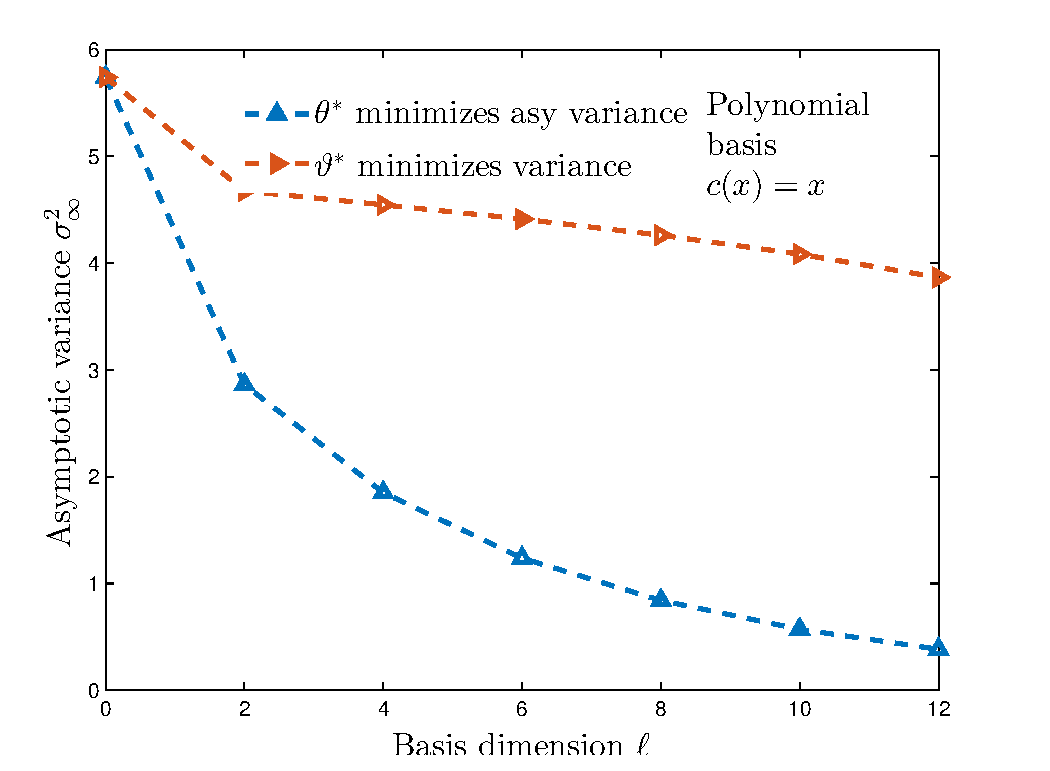
\includegraphics[width=3in]{images/Chap5_x_var_vs_asym_var_poly}} \quad
	\subfigure[]{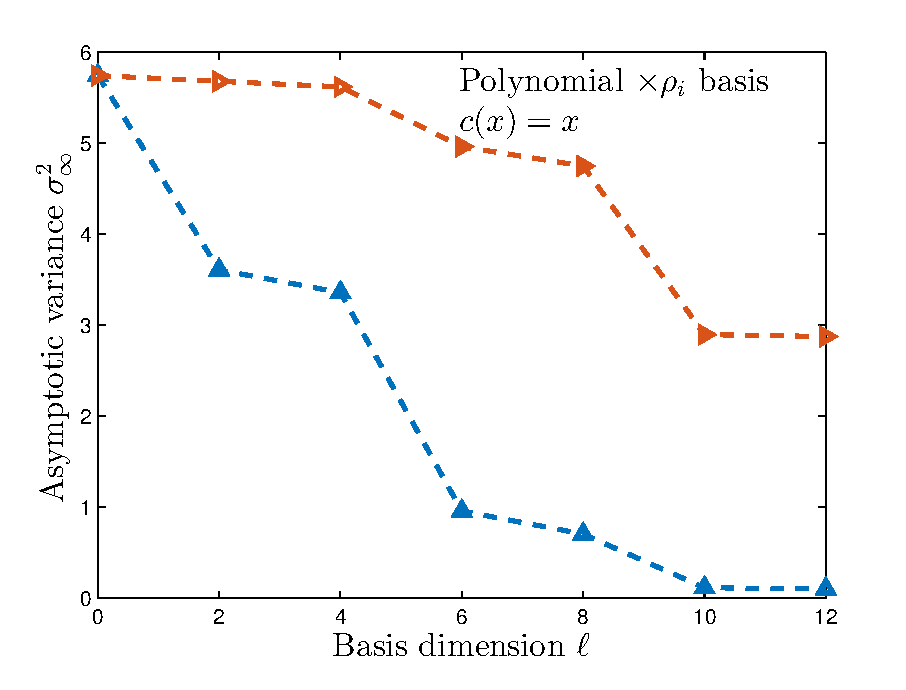
\includegraphics[width=3in]{images/Chap5_x_var_vs_asym_var_wt_poly}}
	% \subfigure[]{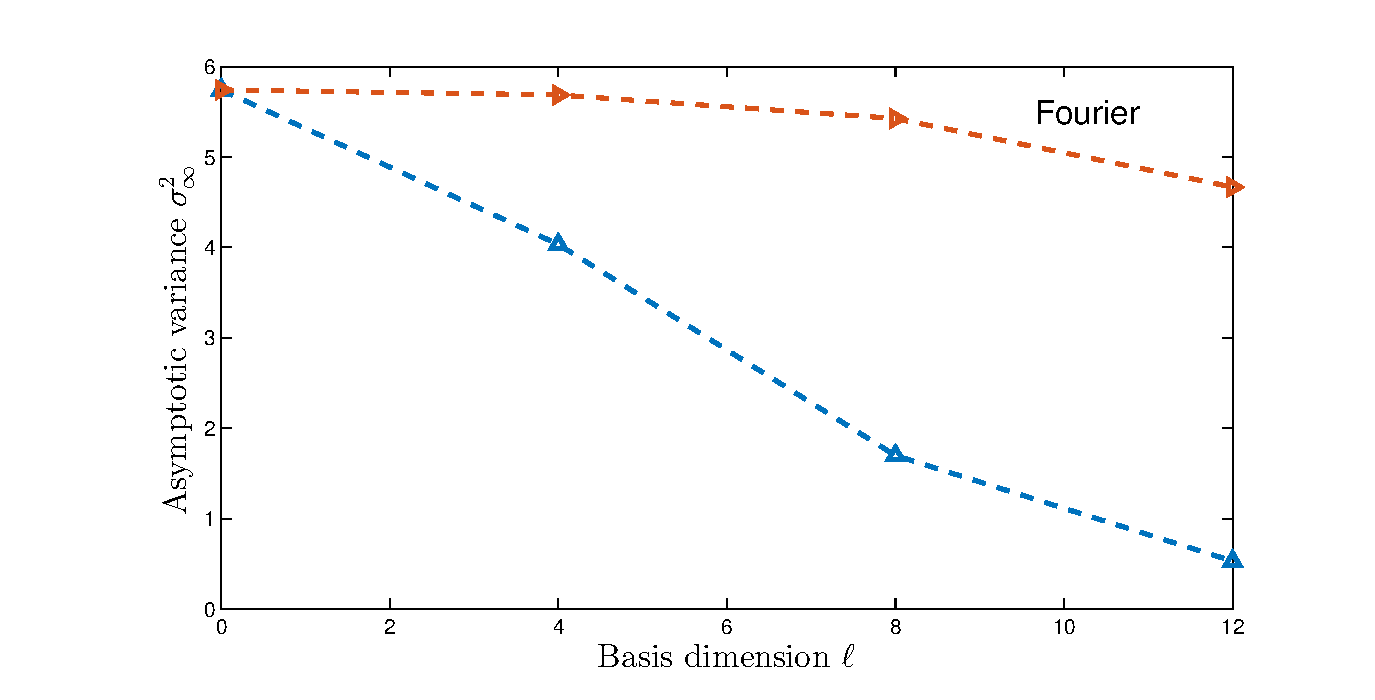
\includegraphics[width=3in]{images/Chap5_x_var_vs_asym_var_fourier}} 
	}

	\mbox{
	\subfigure[]{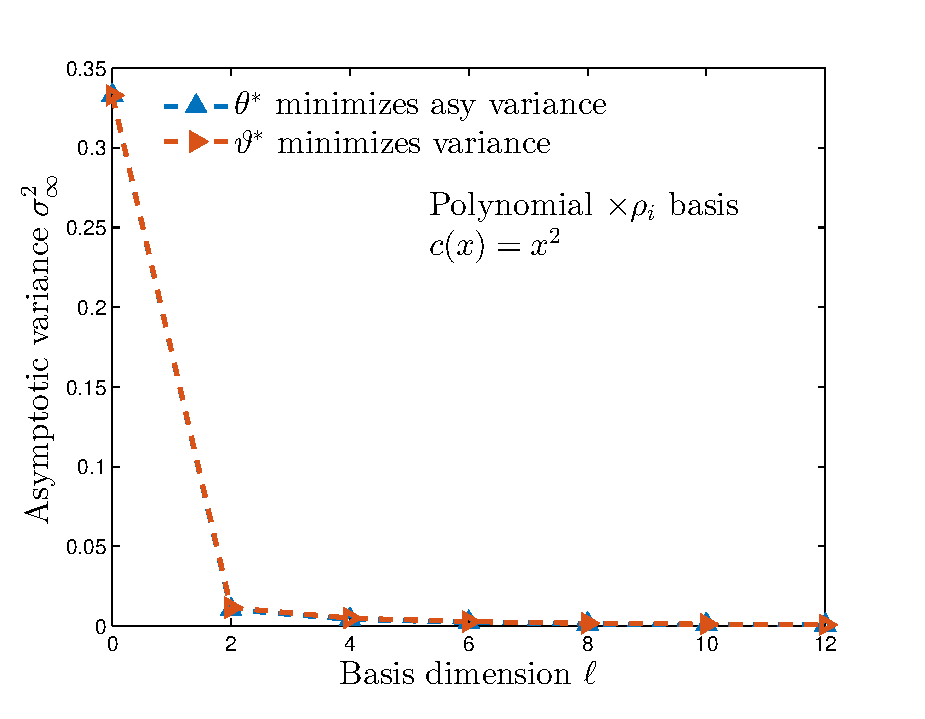
\includegraphics[width=3in]{images/Chap5_x2_var_vs_asym_var_poly}} \quad
	\subfigure[]{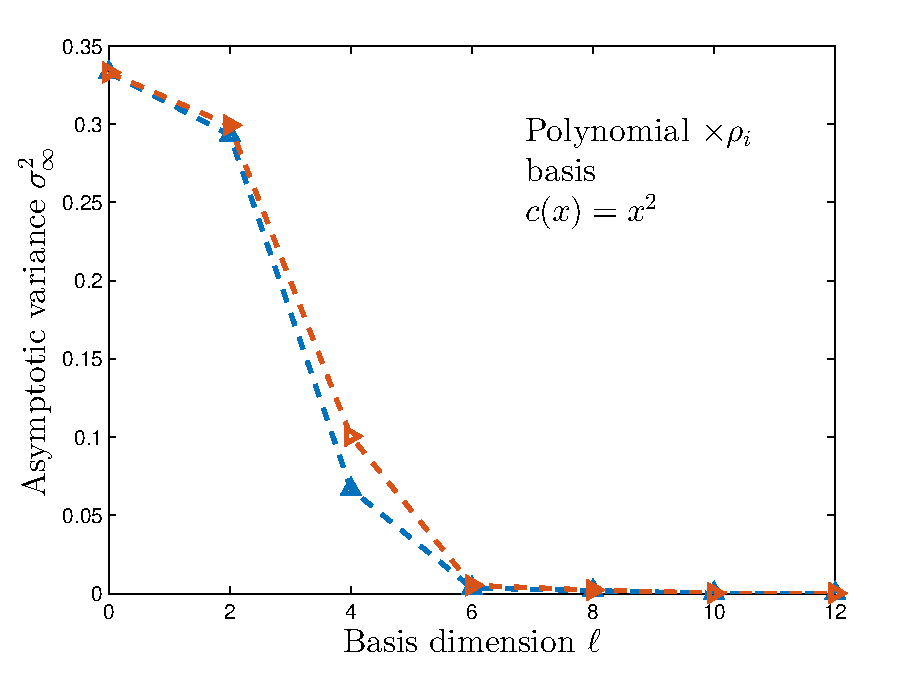
\includegraphics[width=3in]{images/Chap5_x2_var_vs_asym_var_wt_poly}}
	% \subfigure[]{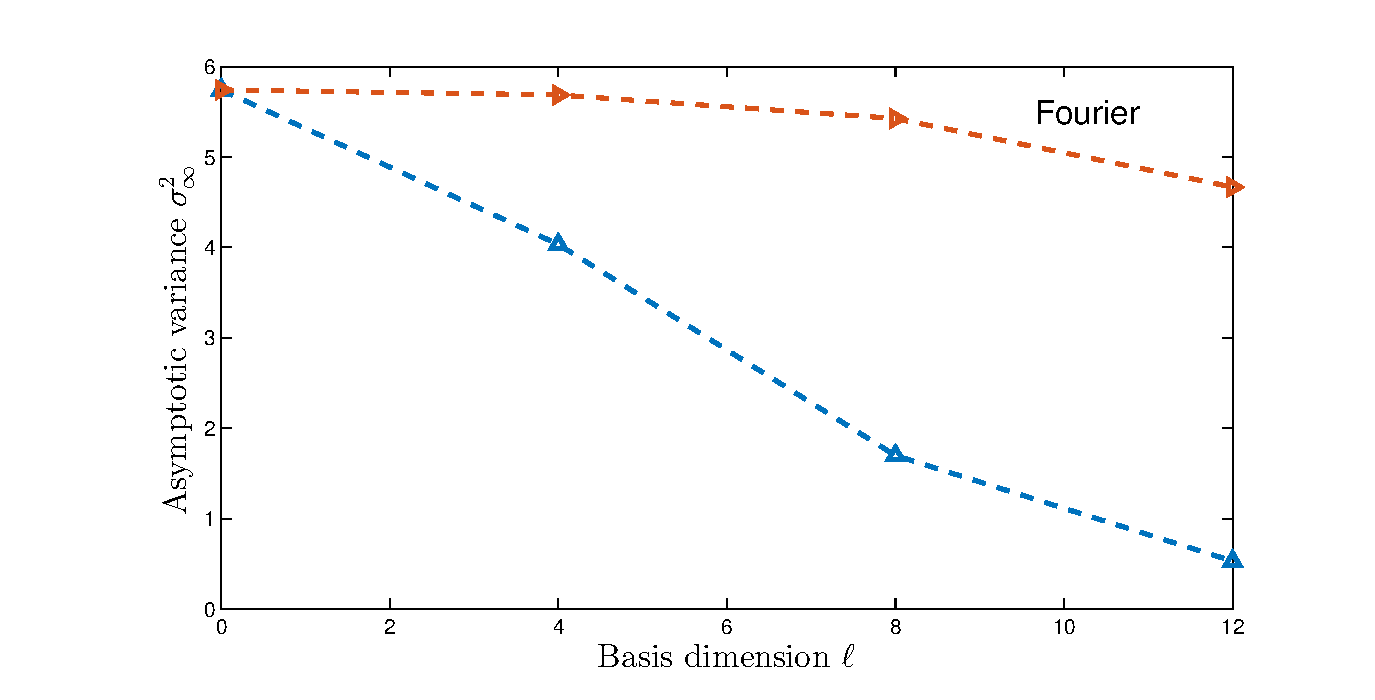
\includegraphics[width=3in]{images/Chap5_x_var_vs_asym_var_fourier}} 
	}
	\caption{Comparison of $(\asymvar^{\theta^*})^2$ and $(\asymvar^{\vartheta^*})^2$}
	\label{fig:mcmc_var_vs_asym_var}
\end{figure}

The discrepancy is clear from a close look at the two functions $c^{\theta^*}$ and $c^{\vartheta^*}$ that are plotted
in \Fig{fig:mcmc_cv_theta_var}.    The key difference is that the ``local mean'' of $c^{\theta^*}$ is nearly $\eta$ in each well of the density $\pr$ (shaded region of \Fig{fig:mcmc_cv_theta_var}):
\[
\begin{aligned}
\int_{-\infty}^0 c^{\theta^*}(x) \pr(x)\, dx	
\approx
\int_0^\infty c^{\theta^*}(x) \pr(x) \, dx \approx \eta =0
\end{aligned}
\]
This helps reduce the asymptotic variance for this slowly mixing diffusion. The function $c^{\vartheta^*}$  does not share this property and produces biased estimates of $\eta$ in each well.
The approximations $h'^{\vartheta^*}$ and $h'^{\theta^*}$ are plotted along with the exact solution $h'$ obtained analytically in
\Fig{fig:mcmc_cv_theta_var}.  The function $h'^{\vartheta^*}$ is a poor approximation to $h'$,  and that results in much higher asymptotic variance. In summary, to minimize the asymptotic variance, it is  important to approximate $h'$ quite well and our objective function aims to minimize the approximation error in the mean-square sense. The same experiment was repeated for $c(x) \equiv\sin x$ with similar results. However, for $c(x) = x^2$, both the methods achieve nearly similar reduction in asymptotic variance. 

\begin{figure}[htbp]
	\centering
	\mbox{
		\subfigure []	{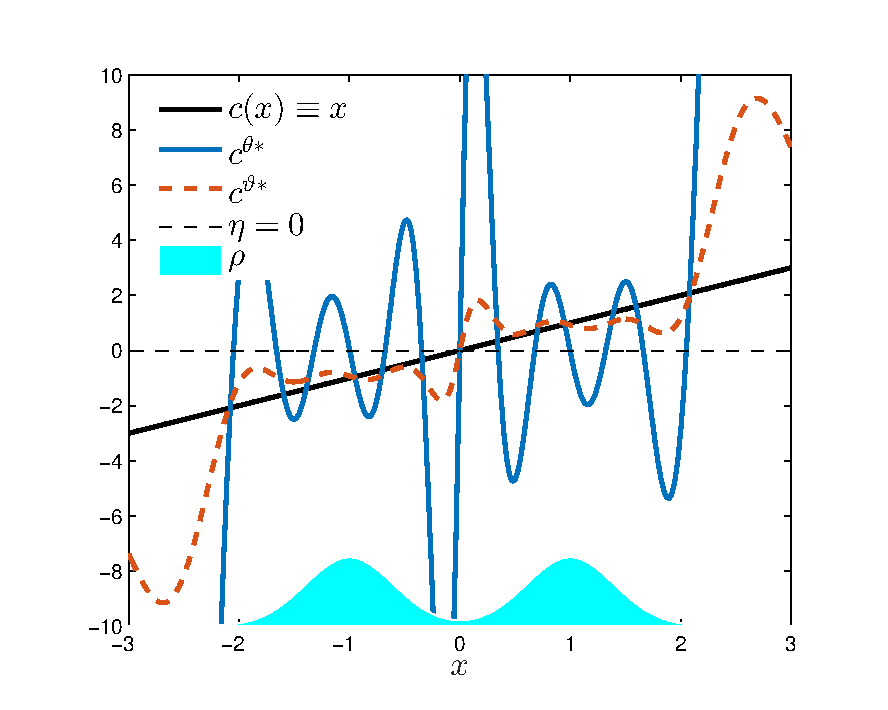
\includegraphics[width=3in]{images/Chap5_x_cvs}} \quad
		\subfigure [] {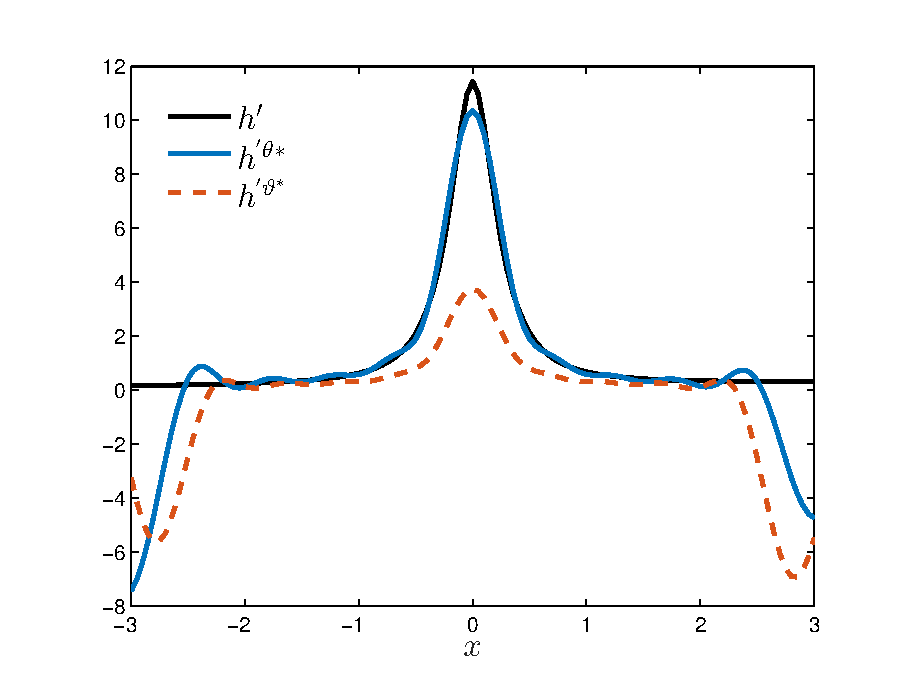
\includegraphics[width=3in]{images/Chap5_x_h_comparison}} 
	}
	\caption{i) Modified estimators using control variates $c^{\theta^*}$ and $c^{\vartheta^*}$, ii) Approximations $h'^{\theta^*}$ and $h'^{\vartheta^*}$ plotted with true gradient $h'$ for $c(x) =x$ with a polynomial $\times \rho_i$ basis.}
	\label{fig:mcmc_cv_theta_var}
\end{figure}


Another way to verify if the two objectives are equivalent is by looking at the autocorrelation functions. In the discrete time case, the asymptotic variance of the estimates of $\eta$ can be written as the infinite sum of all the autocorrelation functions,
\begin{equation}
\begin{aligned}
\asymvar^2  & \eqdef \sum_{n=-\infty}^\infty R(n), \qquad R(n) = \Expect [\tilc(\markovstate) \tilc(\markovstate_n)] \\
& = 2 \sum_{n=0}^\infty R(n)- R(0)
\end{aligned}
\label{e:mcmc_autocorrelation}
\end{equation}
It may be noted that $c^{\theta^*}$ tries to minimize $\asymvar^2$ whereas $c^{\vartheta^*}$ minimizes just a term $R(0)$ in it. \Fig{fig:mcmc_autocorrelation} shows the autocorrelation function $R(n)$ in \eqref{e:mcmc_autocorrelation} corresponding to the three different estimators $c,c^{\theta^*}$  and $c^{\vartheta^*}$ plotted for $n$ upto $100$. Although, $c^{\vartheta^{*}}$ has the least correlation value at $n=0$ (variance), it shows a slow decay as $n$ increases, whereas $c^{\theta^*}$ shows a much steeper decay, resulting in a much lower overall asymptotic variance. The plot clearly illustrates that minimizing the sample variance is not always equivalent to minimizing the asymptotic variance.

\begin{figure}[htbp]
	\centering
	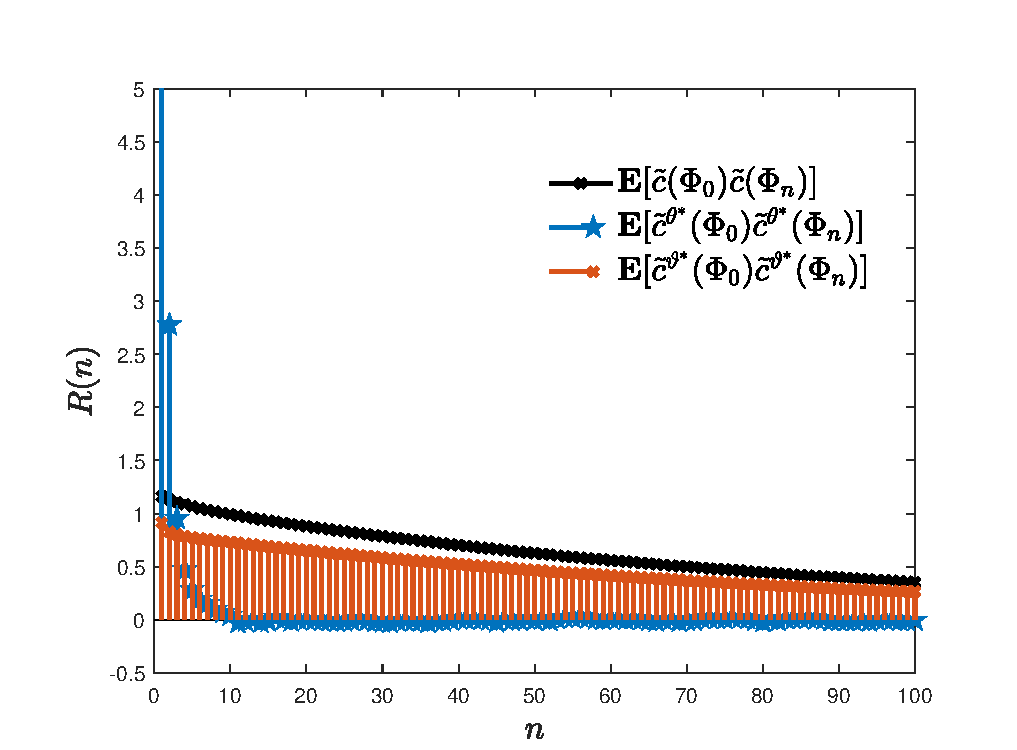
\includegraphics[width=4in]{images/Chap5_cov_R_n_gamma_pt05}
	\caption{ Autocorrelation functions $R(n)$ corresponding to the three estimators $c, c^{\theta^*}$ and $c^{\vartheta^*}$  for $n= 0$ to $100$  }
	\label{fig:mcmc_auto_correlation}
\end{figure}

\section{Numerical Examples}
\label{s:mcmc_numerics}
In this section we present a survey of the numerical experiments performed based on the algorithms presented in this paper. We illustrate the remarkable reduction in asymptotic variance that is achieved by the various $\gradTD$ based algorithms, first on a univariate Gaussian mixture target density and simple functions $c(x)$.   

%\subsection{Asymptotic variance reduction}
%\label{s:ex_avar}
%In this section, we first look at how the control variates help in reducing the asymptotic variance for the unadjusted Langevin algorithm (ULA) \cite{andddefdoujor03}, which is a discrete time approximation of a Langevin diffusion process.  For a simple demonstration of the idea, we consider a one dimensional  multimodal target density defined as mixture of Gaussians \eqref{e:fpf_gaussian_mix}. In our first example, we chose the same parameter values used in \Chapter{ch:fpf} - $M=2$, $\mu_1$ and $\mu_2$ are set to $-1$ and $1$ respectively, $\sigma_1 = \sigma_2 = 0.4472$ and $w_1 = w_2 = 0.5$. This gives a symmetric density $\pr$ as shown by the shaded region in \Fig{cv_theta_var}. The linear function $c(x) \equiv x$ is used in the simulation experiments; symmetry of $\pr$ and $c$ being an odd function imply $\eta = 0$.
%
%First, a finite linear parameterization is adopted, of the form
%\[
%h^\theta(x) =  \sum_{i=1}^\ell \theta_i \psi_i(x)
%\]
%in which $\ell$ is even, and denoting $\ell' = \ell/2$,
%\begin{equation}
%\{\psi_i(x) : x\in\Re,\ 1\le i\le \ell\}  = \{ x^k \pr_m(x) :  0\le k \le \ell',   \ m=1,2\}
%\label{e:basis}
%\end{equation}
%where $\pr_m \sim N(\mu_m, \sigma^2_m)$. The rationale behind this choice of basis functions is that the contribution of each $\psi_i$ is local to a particular mode.  This allows us to approximate $h$ with good accuracy in the region around $\mu_1$ and $\mu_2$, where most of the samples of the Langevin diffusion are concentrated. 
%
%\subsection*{Unadjusted Langevin Algorithm (ULA)}
%The Langevin diffusion process was simulated using Euler discretization with a step size of $0.1$. \Fig{asym_var} shows a comparison of the theoretical reduction in asymptotic variance $\gamma_\theta^2$ with the basis dimension $\ell$, obtained for both basis 1 and 2. The case $\ell=0$ corresponds to the standard Monte Carlo estimator \eqref{e:sample_mean}. The variance decreases significantly from around $7.4$ for $\ell=0$ to $0.12$ for $\ell=20$ for each basis. It can be seen that basis 1 achieves a larger reduction in the asymptotic variance for $2 \leq \ell \leq 16$. In fact, basis 1 with $\ell=6$ gives roughly the same asymptotic variance as basis 2 with $\ell=12$. This shows that choosing an appropriate basis can help achieve the target variance with a much lower basis dimension.
%
%\begin{figure}[htbp]
%	\centering
%  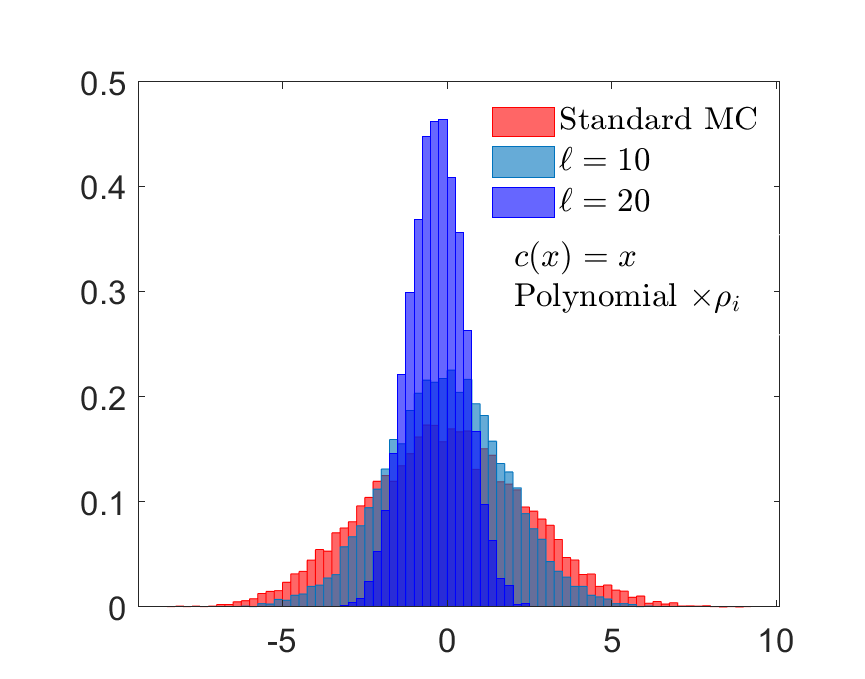
\includegraphics[width=4in]{images/Chap5_hist_all_ds_basis_10000runs_100000samples}
%	\caption{Asymptotic variance reduction in Unadjusted Langevin Algorithm (ULA)}
%	\label{fig:mcmc_ula}
%\end{figure}
%
%
%\Fig{d_all} shows the histograms of the estimates obtained over $10^4$ independent trials for $\ell= 10,20$ compared to the standard MC method. A total number of $10^5$ samples were used in each trial. The empirical variance values observed on the histograms are very close to the analytical variances, although a small bias is seen in the estimate in some cases. This bias may be attributed to the Euler-discretization of the Langevin diffusion which alters the ergodicity properties of the process as mentioned in \cite{robtwe96}.  %\Fig{mean_estimate_lang} compares the trajectories of the mean estimate using the standard ULA technique and the improved estimator with the control variates. The improved estimator shows quicker convergence to the actual mean $\eta$ and far fewer fluctuations than the one using the standard technique.
%
%\begin{figure}[htbp]
%	\centering
%		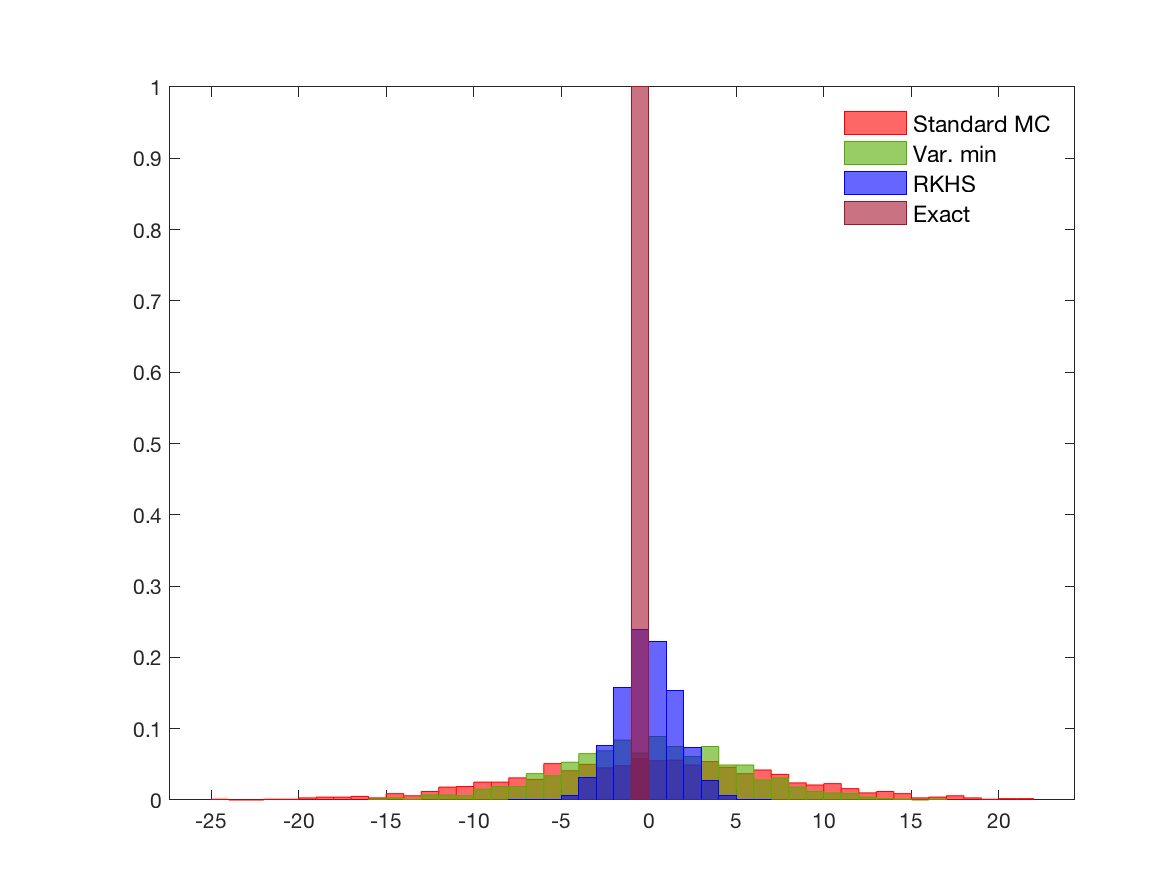
\includegraphics[width=4in]{images/Chap5_hist_asym_var_all_methods}
%		\caption{Histogram of $\sqrt{N}(\eta_N^{i} - \eta$) for the various control variate schemes}
%		\label{hist_all}
%\end{figure}
%
%\Fig{hist_all} presents a comparison of the performance of the control variates obtained by the other approximation schemes that are not based on finite parameterization for the ULA. The histograms were obtained from $1000$ independent trials and the number of samples used in each trial was $N=10^5$. It may be noted that using the exact $h'$ obtained analytically produces a near-zero asymptotic variance. Among the other methods, the RKHS based approximation produces the lowest asymptotic variance. Compared to the standard estimator, the variance minimization method (ZV) \cite{papmirgir14} produced nearly the same variance. Markov semigroup approximation method \cite{tagmeh16a} and the constant approximation to $h'$ produced variance larger the the standard Langevin sampling.
%
%

%In the numerical results discussed, the optimal $\theta^*$ obtained in \eqref{e:theta_star} based on \Prop{t:gradDual} is used. The target density $\pr$ is the same multimodal density as in the previous example. The control variate and the function $c^\theta$ are constructed in the same manner as before, using the same linear parameterization for $h^\theta$. The caveat in this case is that, it cannot be proved that the control variate thus computed is optimal for the RWM algorithm, as \Prop{t:gradDual} is specific to the Langevin diffusion. However, significant reduction in the variance is observed in simulation results. % The intuitive explanation is because of the fact that in the design of $c^\theta$, we try to track $c$ closely using $\generate h^\theta$. Minimizing the error between $h$ and $h^\theta$ tends to minimize the asymptotic variance. In the case of  perfect tracking, $c^\theta$ reduces to the exact mean $\eta$.
%
%\begin{figure}[htbp]
%	\centering
%	\mbox{
%		\subfigure [] {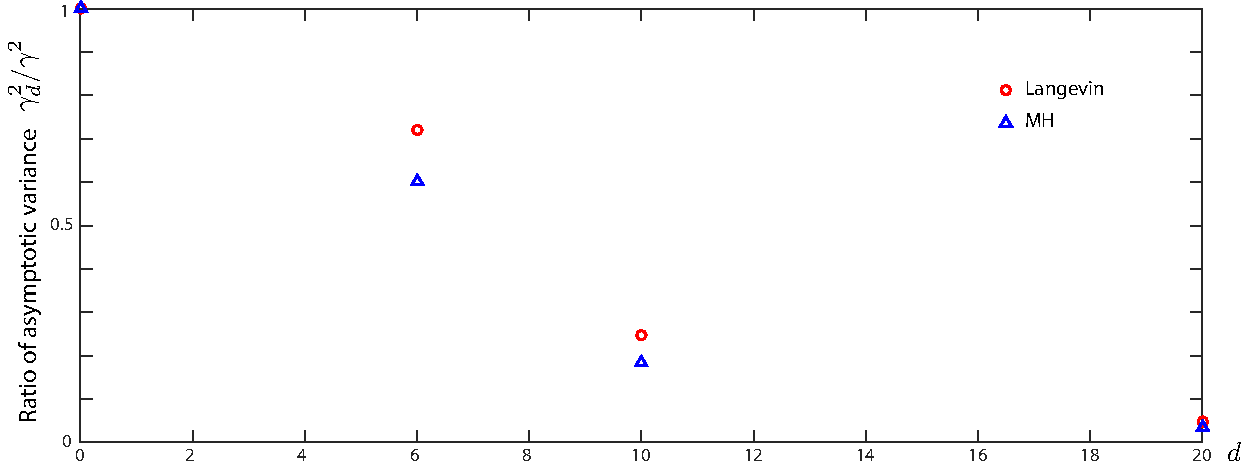
\includegraphics[width=3in]{images/Chap5_rel_red_lang_mh_all}} \qquad
%		\subfigure [] {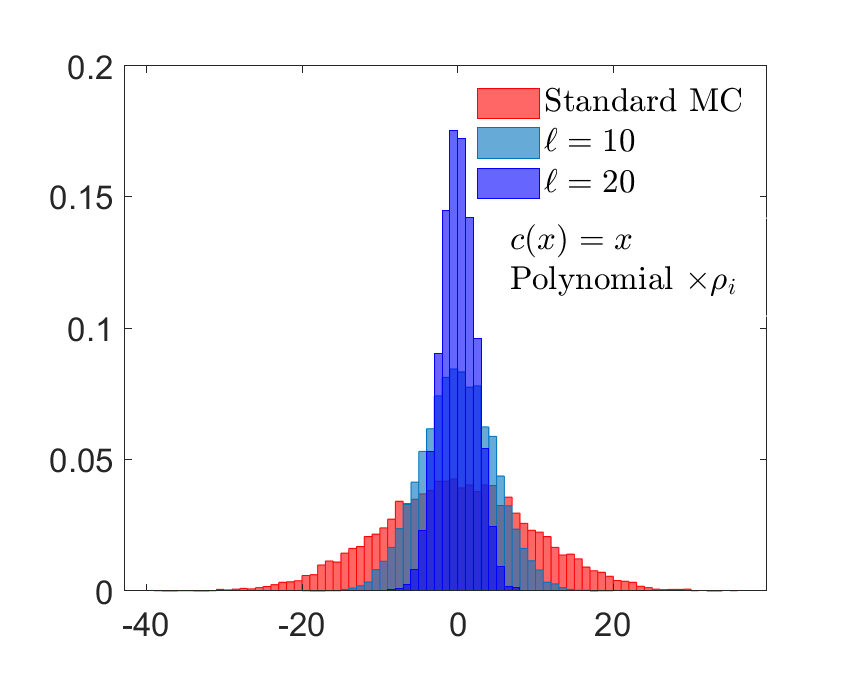
\includegraphics[width = 3in]{images/Chap5_hist_mh_all_ds_basis_10000runs_100000samples}} 
%	} 
%\caption{Asymptotic variance reduction in Metropolis-Hastings algorithm - A) Langevin v Metropolis-Hastings, B) Histogram of $\sqrt{N}(\eta^{i}_N - \eta$) for $\ell=0,10,20$}
%\label{fig:mcmc_metropolis}
%\end{figure}
%
%
%\begin{figure}[htbp]
%	\centering
%		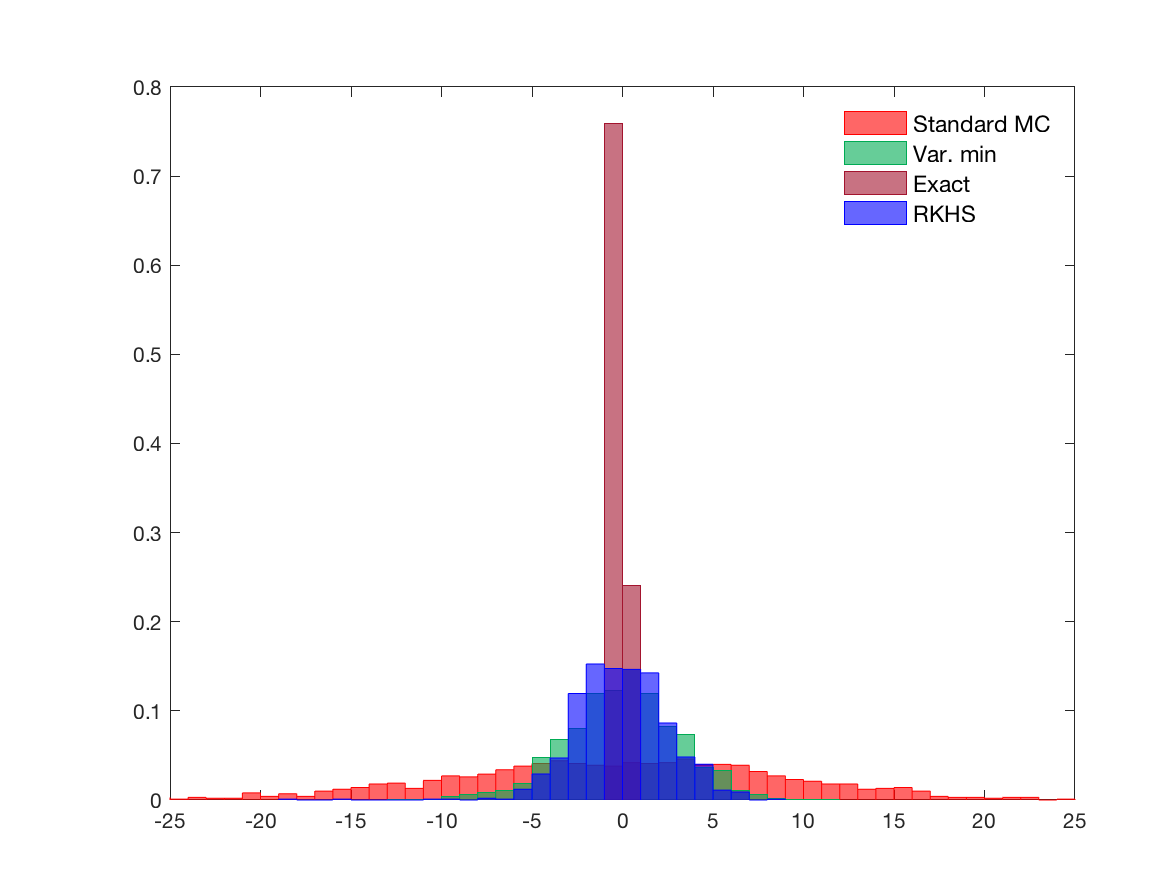
\includegraphics[width=4in]{images/Chap5_hist_mh_asym_var_all_methods}
%		\caption{Histogram of $\sqrt{N}(\eta_N^{i} - \eta$) for the various control variate schemes}
%		\label{hist_mh_all}
%\end{figure}
%\Fig{mh_all} compares the histograms of the estimates of $\eta$ obtained from $1000$ independent runs for $\ell = 6, 10$ and $20$. The histograms show zero-bias and a significant reduction in variance. \Fig{lang_mh} shows the relative reduction in variance for both the ULA and RWM algorithms. The value corresponding to $\ell = 0$ is normalized to $1$ in both the cases. It may be seen that significant variance reduction is achieved for RWM, although at a reduced rate than for ULA.
%
%The algorithm can be applied to a wider class of densities with similar results; we have seen positive results for heavy-tailed densities also. %  Similar trends can also be observed in the Metropolis-Hastings case. \rd{Better results are expected for the Metropolis-Hastings example by applying the algorithm described in \Section{s:cv_reversible_mc}.}
%
%\subsection*{Logistic regression - Swiss bank notes example}
%In practice, MCMC algorithms find wide applications in Bayesian inference problems, where estimates of the mean with respect to the posterior distribution is required. In this section, we discuss a particular example of Bayesian logistic regression or the logit model. A detailed description of the problem in the context of the Swiss bank notes example is given in \cite{papmirgir14} and a brief summary is provided here.
%
%The aim is to learn the regression coefficients that can be used to classify the Swiss bank notes dataset into genuine and counterfeit. Given in the dataset is the measurements for four covariates - the length of the bill, the width of the left and the right edges and the bottom margin width for 200 bank notes of which 100 each are counterfeit and genuine.
%
%Let $X \in \Re^{N_n \times N_d}$ correspond to the covariates measurements of $N_n = 200$ bank notes, with $N_d =4$ denoting the %\notes{ need a new symbol instead of $d$}
%number of covariates. Let $\{Y_i  \in \{0,1\}, 1 \leq i \leq N_n \}$ correspond to the labels for each note being genuine or counterfeit respectively. Let $\boldsymbol{\Theta} \in \Re^{N_d}$ be the regression coefficients that are learned from the given data to obtain a good classifier. We are interested in finding the best estimates for the regression coefficients, i.e. the coefficients that maximize the posterior probability $\pr$ defined as,
%\[
%\pr(\boldsymbol{\Theta}| \{X_i,Y_i\}_{i=1}^{N_n}) \propto \exp\left( \sum_{i=1}^{N_n} \{Y_i \boldsymbol{\Theta}^\transpose X_i - \log(1+e^{\boldsymbol{\Theta}^\transpose X_i} ) \} - 2^{-1} \boldsymbol{\Theta}^\transpose \Sigma^{-1} \boldsymbol{\Theta} \right),
%\]
%where the parameter $\boldsymbol{\Theta} = [ \Theta_1 \dots \Theta_{N_d}]$ has a zero-mean Gaussian prior with a covariance matrix $\Sigma$.
%
%In problems such as this, the maximum likelihood estimate is rarely available in closed-form and is hard to compute. Obtaining the Bayesian estimator requires sampling $\boldsymbol{\Theta}$ values from the posterior distribution and then computing the empirical mean $\hat{\boldsymbol{\Theta}}$. Samples from this posterior density may be obtained using any MCMC technique, in particular we focus on the random walk Metropolis algorithm. In the following, it is assumed that $N$ samples generated by the RWM algorithm are available.
%
%The goal as before is to compute the optimal control variates that minimize the asymptotic variance of the estimate $\hat{\boldsymbol{\Theta}}$.
%Finding the optimal control variates boils down to finding approximate  solutions to the Poisson's equations corresponding to each of the four regression coefficients. The equations to be solved are,
%\begin{equation}
%\generate h_k = -\tilde{\Theta}_k = - (\Theta_k - \hat{\Theta}_k), \qquad \forall k = 1 \dots N_d.
%\label{e:poisson_logit}
%\end{equation}
%The approximation $h^\theta_k$ is chosen to belong to a family of linearly parameterized functions as before,
%\[
%h^\theta_k \eqdef \theta_k^\transpose \psi =  \sum_{j=1}^\ell \theta_{kj} \psi_j,
%\]
%where $\psi_j : \Re^{N_d} \to \Re$ is the chosen set of basis functions and $\theta_{kj} \in \Re$ are the parameter values.  The optimal parameter values are obtained by minimizing $ \| \nabla h_k - \nabla h^\theta_k \|^2_{L^2}$. For a general basis, the optimal parameter $\theta_k^*$  can be derived along the same lines as before,
%\begin{equation}
%\begin{aligned}
%\theta_k^*  &= M^{-1} b_k, \qquad \text{where,}\\
%M & \eqdef \langle \nabla \psi, \nabla \psi \rangle_{L^2} \approx \frac{1}{N} \sum_{i = 0}^{N-1}\nabla \psi(\boldsymbol{\Theta}^i) \nabla \psi^\transpose(\boldsymbol{\Theta}^i)\\
%b_k & \eqdef \langle \tilde{\Theta}_k, \psi \rangle_{L^2} \approx \frac{1}{N} \sum_{i=0}^{N-1}\tilde{\Theta}_k^i \psi(\boldsymbol{\Theta}^i) \\
%\label{e:theta_k}
%\end{aligned}
%\end{equation}
%\noindent \subsubsection*{Linear polynomial basis}
%First we choose $\ell=4$ and $\psi_j$ to be polynomial of degree $1$ as in \cite{papmirgir14}, i.e.
%\[
%\psi^\transpose \eqdef [ \Theta_1 \quad \Theta_2 \quad \Theta_3 \quad \Theta_4] := \boldsymbol{\Theta}^\transpose
%\]
%For this choice of $\psi$,  $\nabla \psi = I$ and $ \Delta \psi = 0$. Hence, $\theta^*_k$ has the simple expression,
%\begin{equation}
%\theta^*_k = \frac{1}{N} \sum_{i=0}^{N-1} \tilde{\Theta}_k^i \boldsymbol{\Theta}^i
%\label{e:theta_lin_polynomial}
%\end{equation}
%The control variate $\generate h^\theta_k$ is explicitly computable and is given by,
%\[
%\generate h^\theta_k(\boldsymbol{\Theta}^i) = -\nabla \log(\pr(\boldsymbol{\Theta}^i|\{X_j,Y_j\}_{j=1}^N)) \cdot \theta^*_k \qquad \forall k, i
%\]
%and the new estimator of the regression coefficients will be,
%\[
%\bar{\Theta}^i_k \eqdef \Theta^i_k + \generate h^\theta_k(\boldsymbol{\Theta}^i).
%\]
%
%As mentioned previously, the \textit{Zero-variance (ZV)} algorithm is proposed in \cite{papmirgir14}  that minimizes the ordinary variance instead of the asymptotic variance. Although it is an easier optimization problem to solve, It is interesting to note that $\theta_k^*$  using \eqref{e:theta_lin_polynomial} is simpler to compute and the solution is numerically more stable (as inversion of an ill-conditioned matrix is not required) than the ZV method.
%\noindent \subsubsection*{Quadratic basis}
%A quadratic polynomial basis of the form,
%\[\psi^\transpose \eqdef [\Theta_1 \quad \Theta_2 \quad \Theta_3 \quad \Theta_4 \quad \Theta_1^2 \quad \Theta_1 \Theta_2 \quad \Theta_1\Theta_3 \quad \Theta_1 \Theta_4 \quad \Theta_2^2 \quad \Theta_2\Theta_3 \quad \Theta_2\Theta_4 \quad \Theta_3^2 \quad \Theta_3 \Theta_4 \quad \Theta_4^2] \]
%is also considered similar to \cite{papmirgir14}.  In this case, $\nabla \psi \in \Re^{14 \times 4}$ and $\theta_k \in \Re^{14}$. The optimal parameter values are given by \eqref{e:theta_k}.
%
%\noindent \subsubsection*{Using RKHS method}
%We also investigate the performance of the RKHS based differential-TD learning algorithm for this example.  The parameter values of $\lambda = 10^{-7}$ and $\epsy = 2$ were found to produce the best results.  Gaussian kernels were placed at $200$ randomly chosen samples.
%
%Simulations were performed using the Swiss bank note dataset provided in \cite{papmirgir14}. We performed $1000$ independent trials each with  $10^5$ samples and $10^4$ samples used for burn-in. The box plots of the estimates of the four regression coefficients $\boldsymbol{\Theta}$ shown in \Fig{Theta_1} - \ref{Theta_4} indicate that significant variance reduction is  achieved using all the control variate methods. It may be observed that for a linear basis, both the ZV and differential TD learning method produce nearly the same asymptotic variance. Using linear polynomials produces values that are $10-65$ times smaller for the four regression coefficient estimates than the standard RWM sampling. For the quadratic polynomial basis, although ZV  outperforms the differential-TD learning method slightly a reduction by a factor of $100-200$ over the standard estimator is still observed. The RKHS method exhibits the best results with variances that are lower by a factor $20-50$ over the ZV method with quadratic polynomials. The RKHS method however has a larger number of outliers. By a more careful choice of the values for $\lambda,\epsy$ and by placing the kernel functions at more well-chosen samples, better results may be obtained. The problem of hyperparameter selection in the RKHS method is discussed in detail in Section \ref{s:hyperparameter}.
%
%%\begin{figure}[htbp]
%%	\centering
%%	\begin{subfigure}{0.45\textwidth}
%%		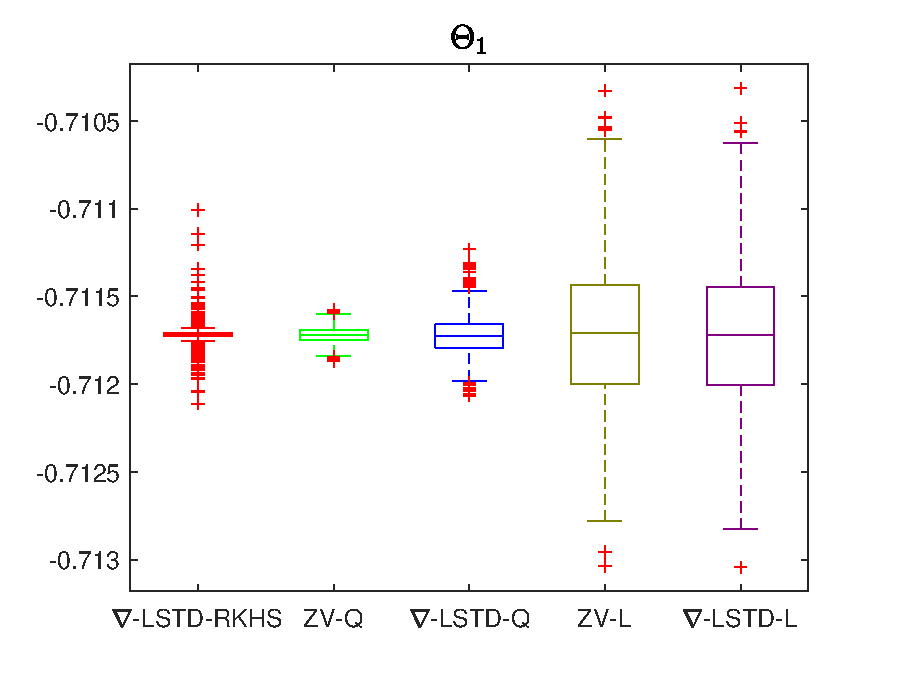
\includegraphics[width=4in]{images/Chap5_hist_Theta1_no_std}
%%		\caption{$\Theta_1$}
%%		\label{Theta_1}
%%	\end{subfigure}
%%	\hfill
%%	\begin{subfigure}{0.45\textwidth}
%%		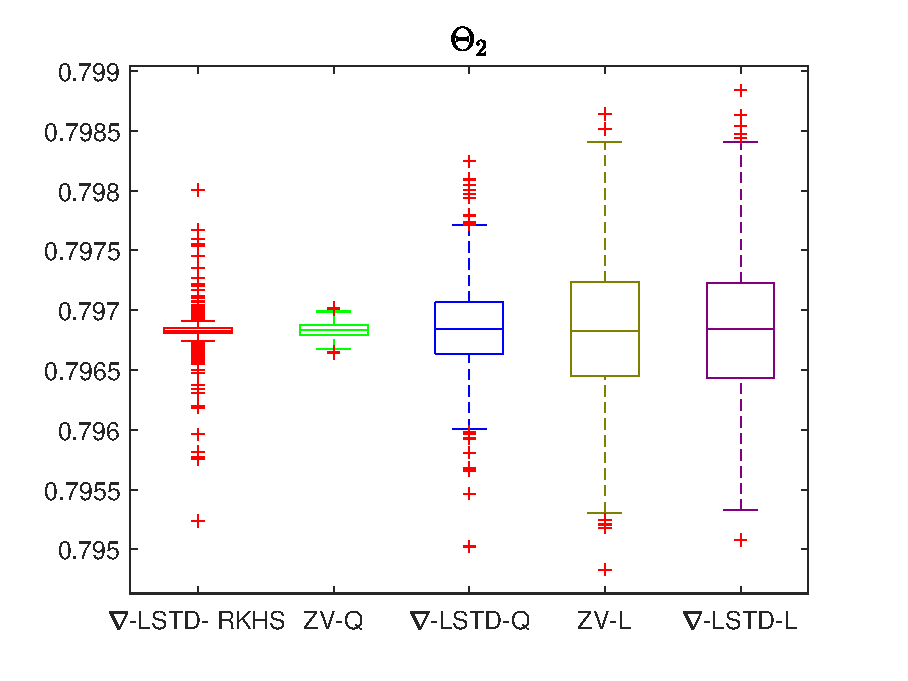
\includegraphics[width=4in]{images/Chap5_hist_Theta2_no_std}
%%		\caption{$\Theta_2$}
%%		\label{Theta_2}
%%	\end{subfigure}
%%	\vfill
%%	\begin{subfigure}{0.45\textwidth}
%%		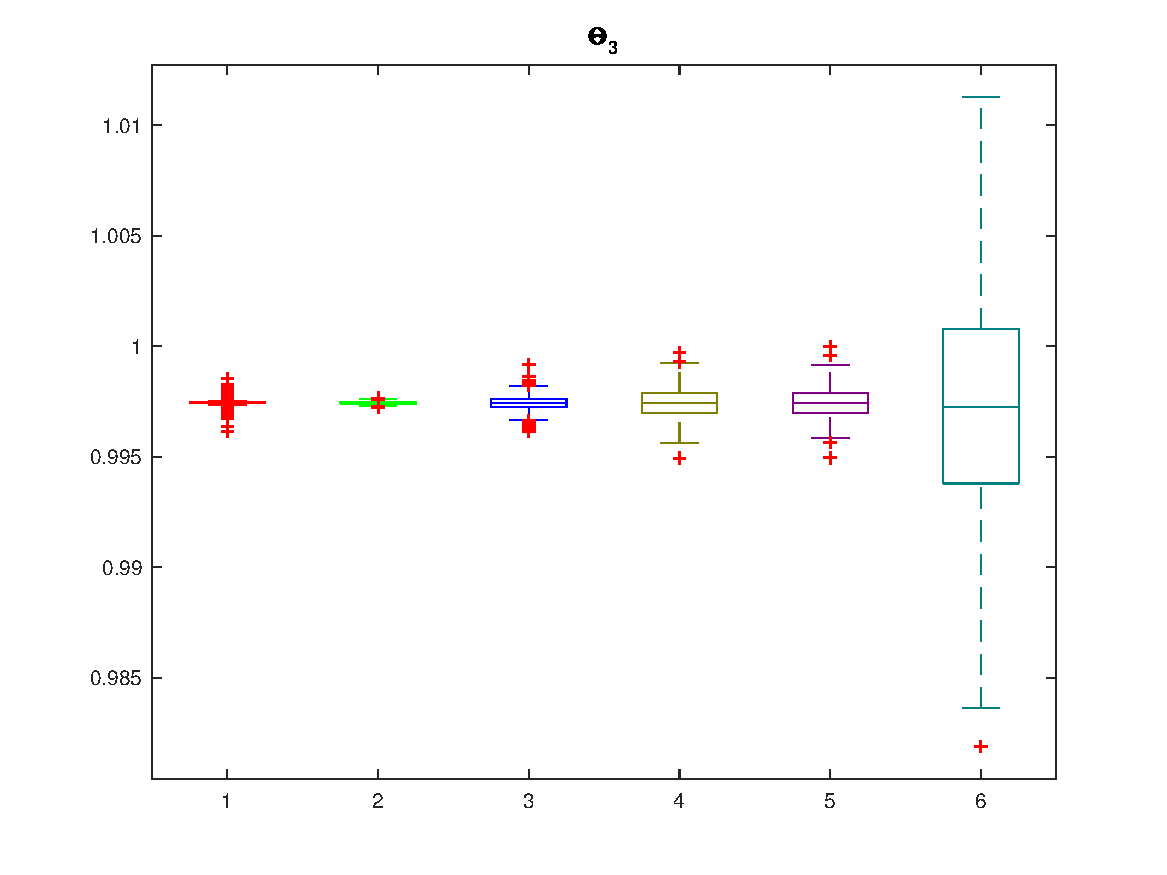
\includegraphics[width=4in]{images/Chap5_hist_Theta3_no_std}
%%		\caption{$\Theta_3$}
%%		\label{Theta_3}
%%	\end{subfigure}
%%	\hfill
%%	\begin{subfigure}{0.45\textwidth}
%%		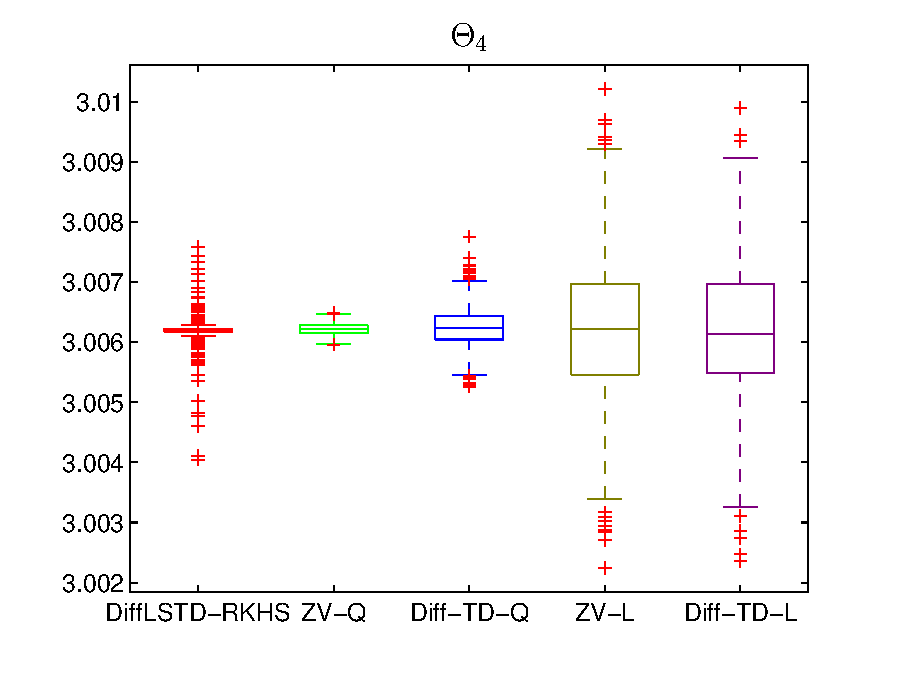
\includegraphics[width=4in]{images/Chap5_hist_Theta4_no_std}
%%		\caption{$\Theta_4$}
%%		\label{Theta_4}
%%	\end{subfigure}
%%	
%%	\label{box_plots_Theta}
%%	\caption{Boxplots of estimates of $\boldsymbol{\Theta}$ obtained over 1000 trials using linear and quadratic polynomial basis (both diff TD learning and ZV-MCMC methods).}
%%\end{figure}
%
%\begin{figure}[htbp]
%	\centering
%	\mbox{
%		\subfigure [] {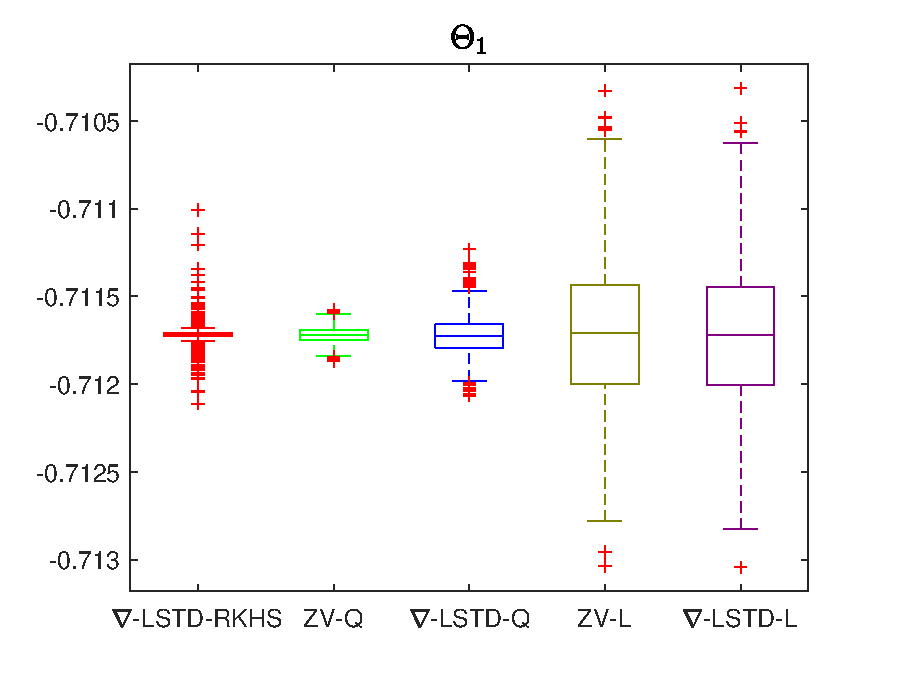
\includegraphics[width=3in]{images/Chap5_hist_Theta1_no_std}} \qquad
%		\subfigure [] {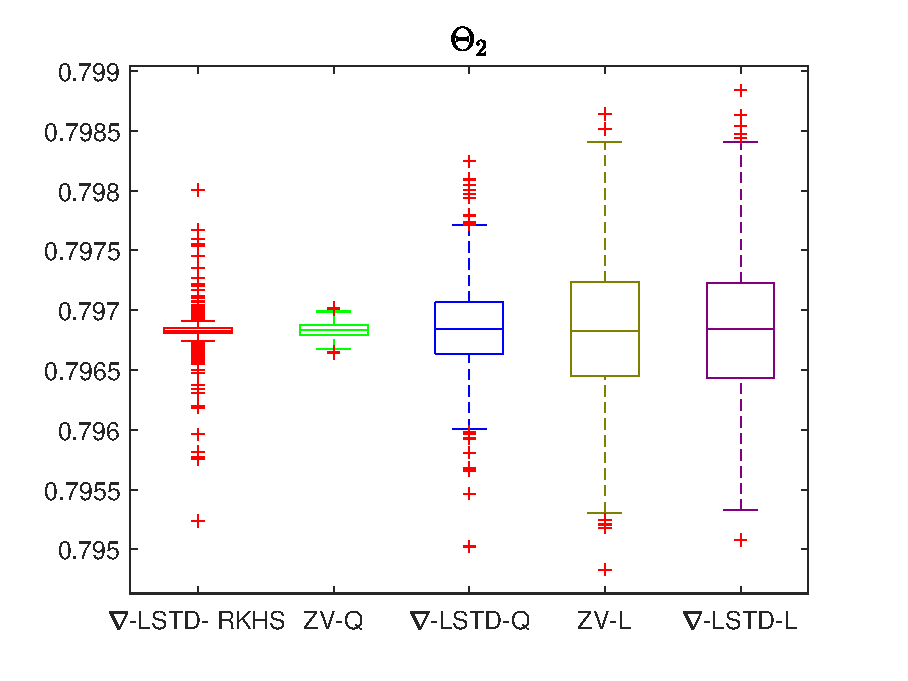
\includegraphics[width=3in]{images/Chap5_hist_Theta2_no_std}} 
%	}
%	\mbox{
%		\subfigure [] {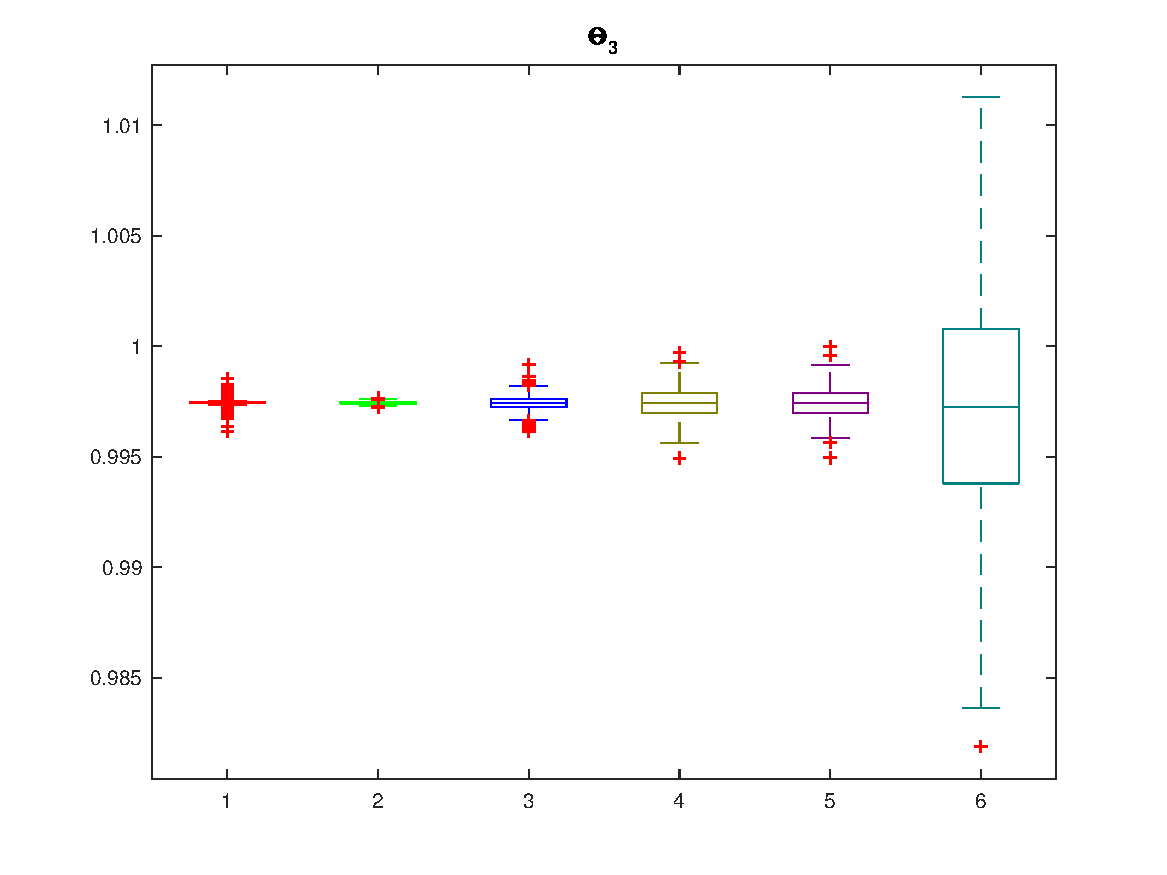
\includegraphics[width = 3in]{images/Chap5_hist_Theta3_no_std}} \qquad
%		\subfigure [] {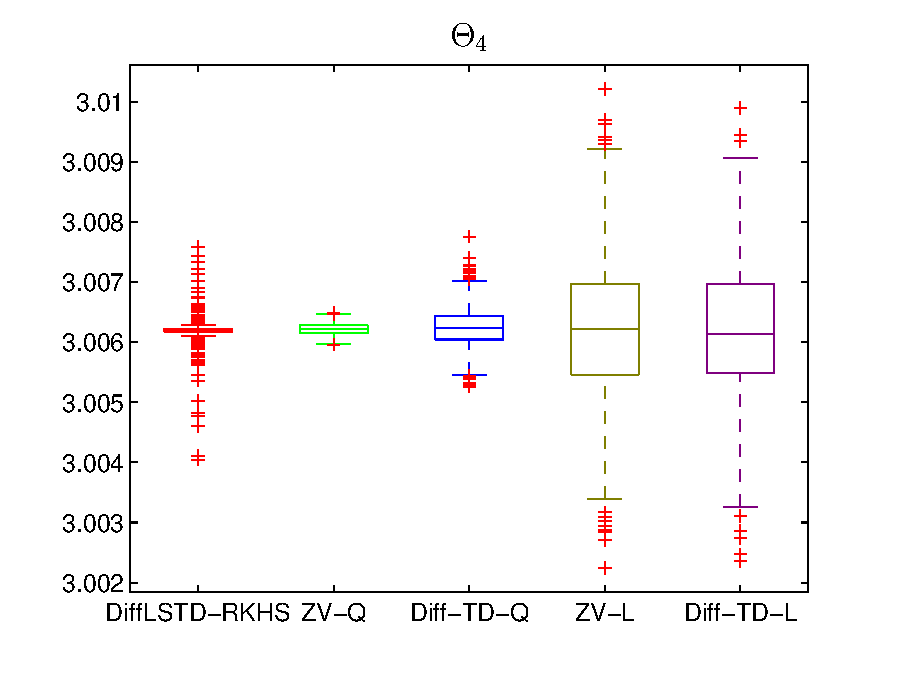
\includegraphics[width = 3in]{images/Chap5_hist_Theta4_no_std}} 
%	} 
%	\caption{Boxplots of estimates of $\boldsymbol{\Theta}$ obtained over 1000 trials using linear and quadratic polynomial basis (both diff TD learning and ZV-MCMC methods).}
%  \label{fig:box_plots_Theta}
%\end{figure}
%
%One might also be interested in the ordinary variance of the samples within a single run. The box plots in \Fig{var_Theta1} - \ref{var_Theta4} compare the variance values of the samples obtained within a run using the ZV method with quadratic polynomials and the RKHS based differential-TD learning method. It may be observed that in spite of having outliers, the mean sample variance using the RKHS method is almost an order of magnitude lower than the ZV method.
%
%The same set of experiments were tried out with similar results for the logistic regression example using MALA and ULA sampling. Similar results were also obtained for the probit model Vaso constriction example discussed in \cite{papmirgir14}. The plots for these simulations are provided in the appendix.
%%\begin{figure}[htbp]
%%	\centering
%%	\begin{subfigure}{0.45\textwidth}
%%		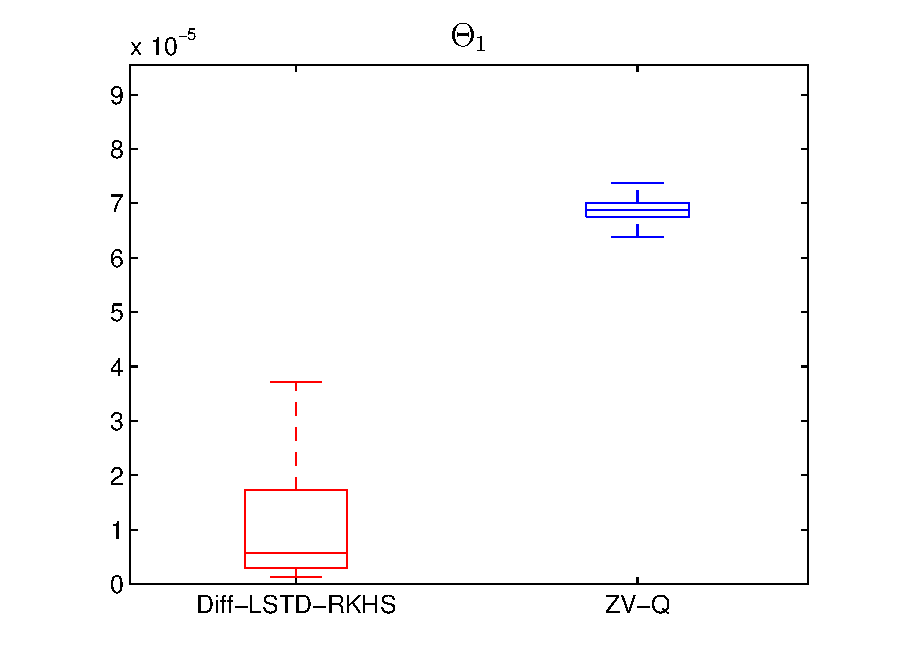
\includegraphics[width=4in]{images/Chap5_box_var_Theta1}
%%		\caption{$\Theta_1$}
%%		\label{var_Theta1}
%%	\end{subfigure}
%%	\hfill
%%	\begin{subfigure}{0.45\textwidth}
%%		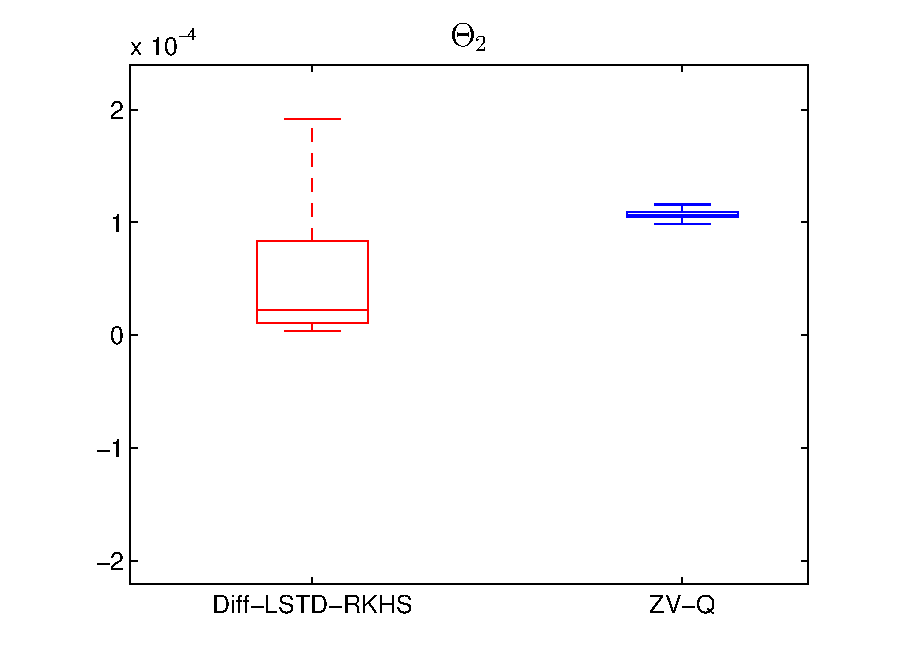
\includegraphics[width=4in]{images/Chap5_box_var_Theta2}
%%		\caption{$\Theta_2$}
%%		\label{var_Theta2}
%%	\end{subfigure}
%%	\vfill
%%	\begin{subfigure}{0.45\textwidth}
%%		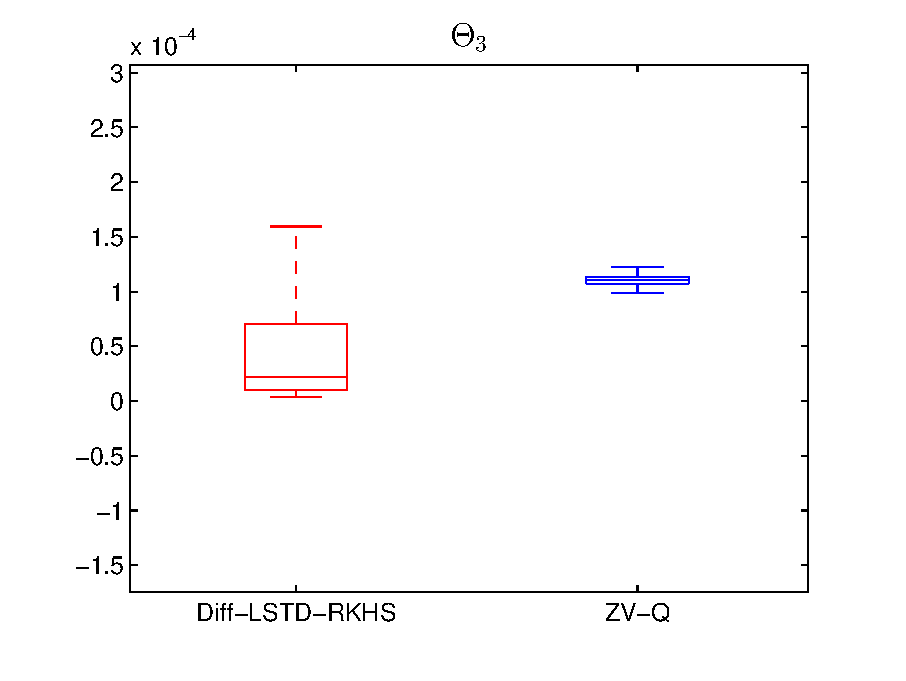
\includegraphics[width=4in]{images/Chap5_box_var_Theta3}
%%		\caption{$\Theta_3$}
%%		\label{var_Theta3}
%%	\end{subfigure}
%%	\hfill
%%	\begin{subfigure}{0.45\textwidth}
%%		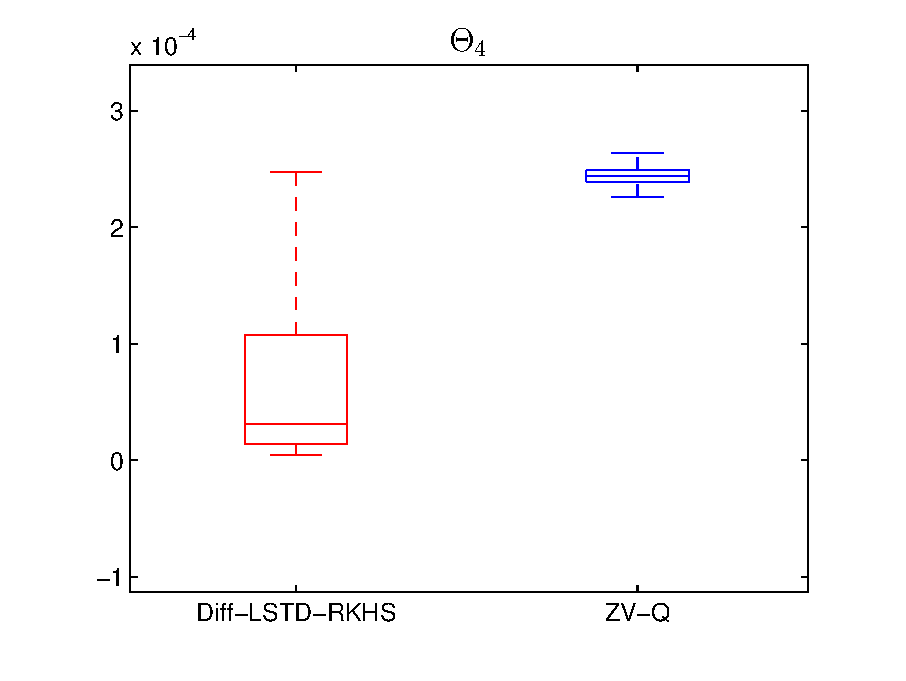
\includegraphics[width=4in]{images/Chap5_box_var_Theta4}
%%		\caption{$\Theta_4$}
%%		\label{var_Theta4}
%%	\end{subfigure}
%	\label{box_plots_ varTheta_all}
%	\caption{Boxplots of the in-trial variances of $\boldsymbol{\Theta}$ obtained over 1000 trials using the differential TD (RKHS) and ZV with quadratic polynomials}
%\end{figure}

%\begin{figure}[htbp]
%	\centering
%	\mbox{
%		\subfigure [] {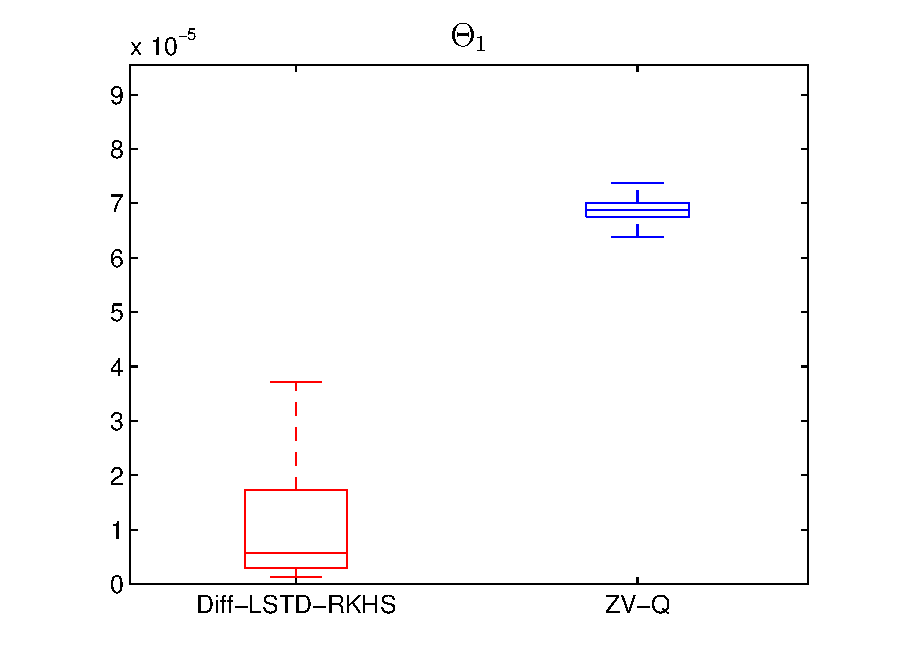
\includegraphics[width=3in]{images/Chap5_box_var_Theta1}} \qquad
%		\subfigure [] {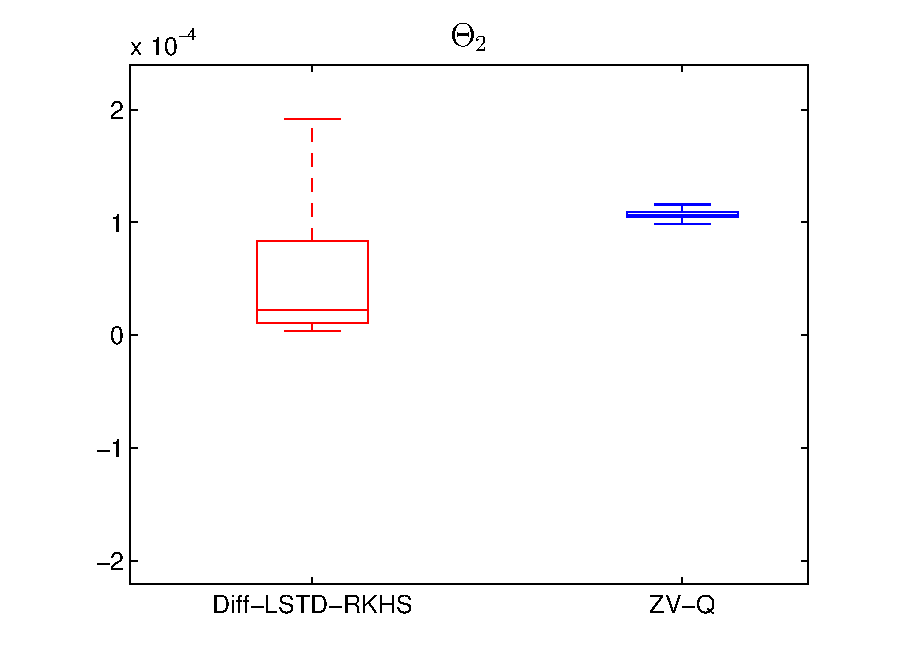
\includegraphics[width=3in]{images/Chap5_box_var_Theta2}} 
%	}
%	\mbox{
%		\subfigure [] {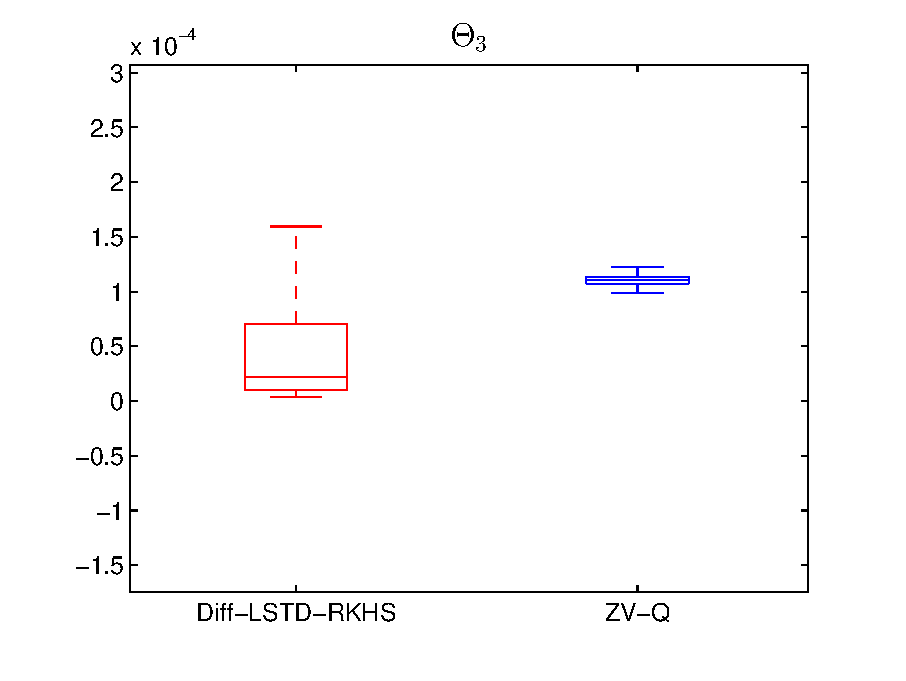
\includegraphics[width = 3in]{images/Chap5_box_var_Theta3}}  \qquad
%		\subfigure [] {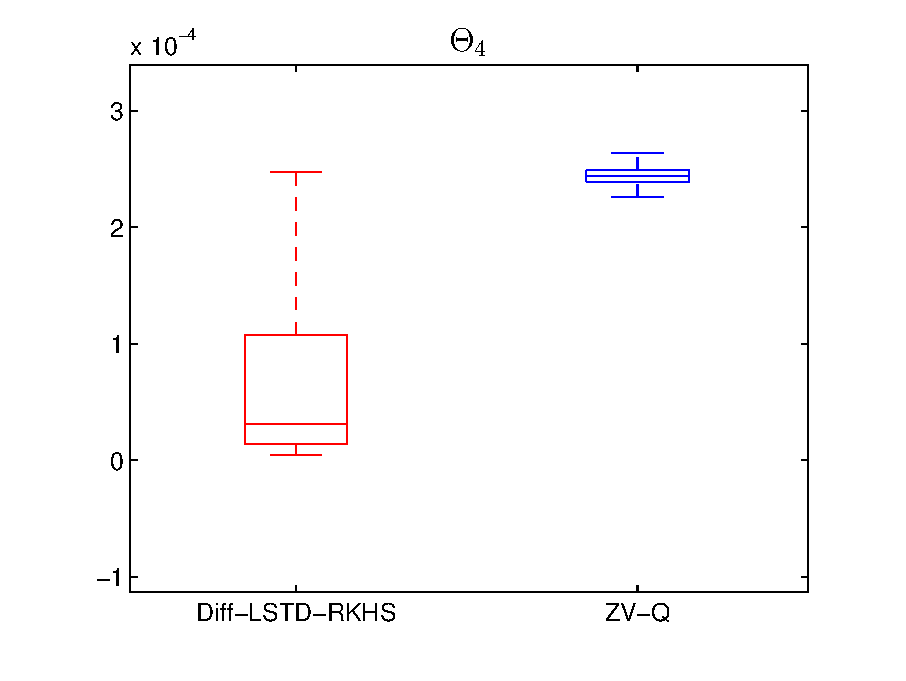
\includegraphics[width = 3in]{images/Chap5_box_var_Theta4}} 
%	} 
%\caption{Boxplots of the in-trial variances of $\boldsymbol{\Theta}$ obtained over 1000 trials using the $\gradTD$-RKHS and ZV with quadratic polynomials}
%\label{fig:mcmc_box_var_Theta}
%\end{figure}
